\documentclass{report}
\usepackage{suthesis-2e}
\dept{Computer Science}

\usepackage[a4paper, total={6in, 8in}]{geometry}

\usepackage{graphics,graphicx,amssymb,amsmath,amsfonts,verbatim}
\usepackage{epsfig}
\usepackage{subfigure}
\usepackage[subnum]{cases}
\usepackage{color}
\usepackage{lineno}
\usepackage{url}
\usepackage{epstopdf}
\epstopdfsetup{update}

\usepackage[utf8]{inputenc}


\usepackage{makeidx}
\makeindex
 

%% CHEMICAL ELEMENTS
\usepackage{chemmacros} 
\chemsetup{modules=all}
\usepackage{chemgreek}

%%  QUOTES
\usepackage{epigraph}
\usepackage{xcolor}
\usepackage{acronym}


\graphicspath{ {img/} }

\title{Tools for heterogeneous diagnostic data integration: application to real-time control of fusion relevant plasmas}
\author{Andrea Rigoni Garola}
\date{July 2019}


%% SUBSTITUTIONS %%
\newcommand{\RFXmod}{RFX-mod}
\newcommand{\Figure}[1]{\textit{Figure}~#1}

%% MATH %%
\newcommand{\transpose}[1]{\ensuremath{#1^{\scriptscriptstyle T}}}
\DeclareMathOperator{\E}{\mathbb{E}}
\newcommand{\expectation}[1]{\ensuremath{\mathbb{E} \left[ #1 \right]}}



\begin{document}
\maketitle
\tableofcontents
\listoffigures
\listoftables

\chapter{Introduction}
\pagenumbering{arabic}

\epigraph{Everyone in a complex system has a slightly different interpretation. The more interpretations we gather, the easier it becomes to gain a sense of the whole.}{Margaret J. Wheatley}


%% - Emerging of Information technology 
How is it possible for the nail size chip in our phone to understand us speaking or to recognize our face among thousands of people? 
It seems like magic that comes from science fiction and in less than a decade has become a contingent reality: every image of all phones is automatically tagged, every face recognized and all conversations typed.
It is not a very surprising fact though that, as a result, many people are actually rising concerns about this growth of technology and even governments are tightening regulations to guarantee the privacy rights against the economic use of people personal information.
%
%% - We can profit of IT for scientific experiment
Nonetheless, beside this new information business, those novel solutions that are mainly pushed by private interests are also very commonly released with open-source licences, thus being available to the scientific community. The idea is that vendors take advantage from a good code quality and the proliferation of new ideas within the wide pool of open-source developers, and at the same time the community gets access to a cheaper hardware and very powerful software tools that can be adapted to any specific need.
%
%% - Data over algorithm -> ML over AI
This new era, led by information theory, is revealing not to emerge from complicate mathematical models but from the data themselves, joined with lower cost per computational operation in terms of energy consumption and components price. %TODO: sistemare %
The predominant role of data is on one side promoting the big infrastructures where huge amount of signals must be collated by efficient databases and promptly passed through analysis algorithms, on the other side it stresses the need of an efficient design of hardware that must be able to adapt to the changes in algorithms and data dimensionality. This transition from single process to big-data analysis matches the shifting interest from the general \ac{AI} approach to the \ac{ML}\footnote{Machine learning is a subset of \acs{AI}. As from the definition by Tom Mitchell, author of the book "Machine Learning": A computer program is said to learn from \textit{experience} $E$ with respect to some class of \textit{tasks} $T$ and \textit{performance} measure $P$ if its performance at \textit{tasks} in $T$, as measured by $P$, improves with experience $E$.}, while from the algorithmic perspective it established the preeminent role of \ac{ANN}.

%% - Experiments may use hard correlated signals
The classical scientific approach is to make hypotheses on an evidence insulating repeatable experimental values and to provide a model able to reproduce those values. But it is not uncommon that within a complex experiment many different systems coexist, each with its own representation model, exposing a non trivial connection with each others. There is also the intuitive perception that gathering more and more information about a phenomenon gives a more accurate representation, but this requires to manage all the possible non-linear correlations coming from the different nature of signals.
~
%% - NN universal approximation
On the other hand it can be proved that any continuous convex function of n-dimensional input variables can be effectively approximated with a n+1 width neural network~\cite{csaji2001approximation}\cite{hanin2017universal}.
%TODO: ESPANDERE %
~
%% - deep learning
The actual turning point in ML happened with the NIPS'12 publishing of AlexNet~\cite{NIPS2012_4824}, a massive GPU trained network that won the ImageNet Large Scale Visual Recognition Challenge\footnote{The ILSVRC (\url{http://www.image-net.org/challenges/LSVRC/}) evaluates algorithms for object detection and image classification at large scale. One high level motivation is to allow researchers to compare progress in detection across a wider variety of objects, taking advantage of the quite expensive labeling effort.} achieving a top-5 error 10.8\% lower than the runner up. 
The original paper's primary result was that the depth of the model was essential for its high performance, opening the era of Deep Learning~\cite{Goodfellow-et-al-2016}.

%% - this thesis data integration using deep learning
A complex and heterogeneous experimental system could then benefit of this methodology in many ways: the possibility to integrate many different kinds of signals, the robustness to react on missing or corrupted data in case a portion of the sensory system fails, and the flexibility to adapt to changes on both the parameters or the environment variables of the experiment.
%
This thesis dissertation will present a set of tools that exploit such data integration, using the deep learning techniques from both the hardware and software perspective, applied to a possible scenario of controlling the magnetic confinement of a nuclear fusion plasma. 
% TODO: add.. in addition we will present the hardware implementation suitable to achieve the task
%
%% this is indeed a complex experimental setup applied to RFX-mod
This is, indeed, a very complex task other than one of the main challenges of this century. In this context the \textit{RFX~consortium} is hosting RFX-mod, one of the most controllable fusion experiments currently active in fusion research~\cite{SONATO2003161}\cite{doi:10.1063/1.4806765}.
Recently a further update to the experiment (RFX-mod2) has begun, aiming to improve the responsiveness of the machine, together with the renew of the sensory system. The research application described in the present work fits in this environment with a specific design proposal that integrates a \ac{ML} based control loop to the overall chain of data acquisition and control.

%TODO: REVIEW DOPO AVER SCRITTO INTRO%
In the next section a brief introduction to the problem of magnetic confinement will be presented followed by a description of the intuitive principles that justify the application of this kind of control.




\section{Magnetic confined nuclear fusion}
% FUSION %
The referred nuclear process is the exothermic reaction that happens between two light atom nuclei that fuse together. A fusion process that produces a transmutation to a new nucleus lighter than iron-56 or nickel-62 generally yields a release of energy. These elements have the smallest mass per nucleon and the largest binding energy; so the fusion of light nuclei toward, as well as fission of elements beyond these elements releases the energy retained, resulting in a exothermic reaction.  This means that, with the purpose of extracting energy, the lighter elements (hydrogen and helium) are in general more likely to be the fusible fuel, while the heavier elements (uranium, thorium and plutonium) are more likely to be the fissionable one. 
Figure~\ref{fig:binding} shows the binding energy per nucleon as a function of the atomic mass number. The exceptional situation of 4 (He) is shown. Fusion processes ending in He show the largest exothermal response; the burning of 1 (H) to 4 (He) releases most of the energy available to fusion. The maximum of the binding energy is with 56 (Fe).
\begin{figure}[ht!]
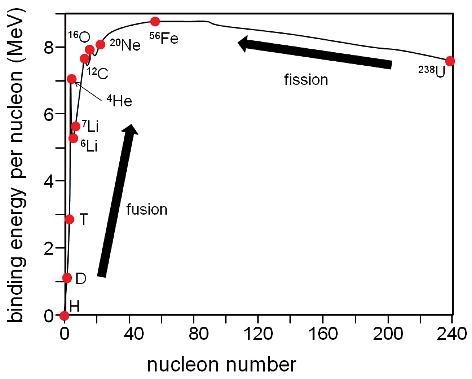
\includegraphics[height=0.25\textwidth]{img/binding_energy.jpg} \centering
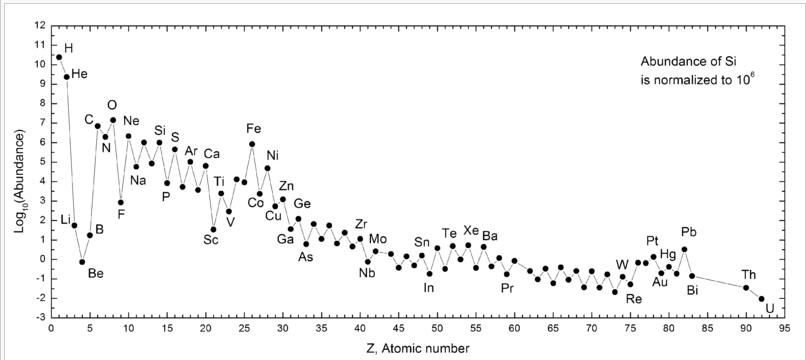
\includegraphics[height=0.25\textwidth]{img/abundance.png} \centering
\caption{Binding energy per nucleon for each element atomic number. }
\label{fig:binding}
\end{figure}

% FUELS and abundancy of elements %
The universe as forged by the Big-Bang was initially mainly formed by leptons along with simple elements: protons, deuterons, and a little quantity of helium and lithium. All the remaining set of the 92 known elements, from carbon up to uranium are afterwards the expression of the self-organisation of the universe - the formation of galaxies where the stars burn hydrogen as breeder material for new elements - enforced by gravity\footnote{ Lithium, Beryllium and Boron are relatively rare in cosmos since they had little time to form in the first expansion and are not directly synthesized by stars; their nuclei are actually destroyed within the star's core, however a small quantity can be produced by break-up of heavier elements in interstellar dust, as a result of impact by cosmic rays\cite{LiBeB_syntesis}}.

% Fusion and Fission in cosmos %
The production of heavy fission fuels by nucleosynthesis is generally ascribed to extreme astrophysical events like supernovas, that are able to reach enough energy to fuse nuclei into elements heavier than iron; when we use nuclear power coming from fission process we are indirectly recovering energy from those relatively rare events.
% 
On the other hand, as stated, the most common spread process in the universe is the burning of Hydrogen in the so called \textit{pp} chain reaction, firstly described by H.Bethe in 1939. 
In the core of a star, gravity produces high density and high temperature. The gas density in the core of our sun is 160 g/cm3, much higher than the densest metal, and the temperature is about $15\times10^6K$ ( $\simeq 1.5 KeV$ ). Under these extreme conditions the kinetic energy of particles and the continuous collisions disentangle all the electrons from the nuclei so the matter appears in the form of plasma. Protons (H-1) react with other protons to make deuterium nuclei (H-2) and positrons. The deuterium nuclei can merge to form a helium nuclei (He-4), or they can interact with other protons to make another isotope of helium (He-3). Two He-3 nuclei can fuse to make a nucleus of an unstable beryllium nucleus (Be-6) that breaks apart to give He-4 and two protons. Energy is released at each step.

In this sense the Hydrogen fusion is the most common way to obtain energy in the cosmos, and it is not by chance that the majority of the earth available energy resources are actually coming from the sun.

% Fusion in earth %
Starting from the Oliphant, Harteck and Rutherford experiments, that in 1934 provided for the first time the proof of transmutation accelerating Hydrogen~\cite{1934RSPSA.144..692O}, the attention quickly moved toward the plasma physics research by means of thermal excitation with the design of the \textit{tokamak} as a magnetic confinement device by the soviet physicists Igor Tamm and Andrei Sakharnov in 1950.%~\cite{}. 
%
% Cross section
% RR 
The fusion process between positively charged nuclei has to overcome the Coulomb repulsion, and the potential energy at a distance of a proton diameter is about 0.6 MeV. Nature eases fusion because the particles (the protons in this case) in this interaction adopt the characteristics of a wave, which allows them to leak into the energetically prohibited zone and to finally tunnel through the Coulomb barrier into the deep bound states of the newly formed nuclei. The potential energy at the distance of the de~Broglie wave length is about two orders of magnitude lower than the one within the range of the nuclear forces. The fusion yield depends on the density of the particles, their relative velocity and the nuclear interaction in the form of the fusion cross-section. 
The interaction processes are Coulomb collisions between charged particles. As the Coulomb collision rate is large compared to the fusion rate, the proton assembly (as well as the one of the electrons) can be described by a Maxwellian distribution. The governing kinetic parameter is the temperature rather than the individual particle energy in the assembly interactions scattering and fusion. This is the reason why we are speaking of controlled thermo-nuclear fusion.

% Lawson and why tokamak
The idea follows the simple principle that we need to produce fusion events at a rate that the system can, at least, virtually self sustain the reaction. 
\cite{Wagner.Friedrich:magnetic.confinement.intro}
The rate of fusion power normalized by the amount of external power needed is typically defined as the \textbf{Q} factor; 
% cross section rates and selection of thermal reaction
The selection of the proper reaction is guided, however, by searching for the highest reaction rate providing the highest fusion yield. This condition is fulfilled by fusing deuterium $D=\isotope{2,H}^+$, the heavy isotope of hydrogen, with tritium $T=\isotope{3,H}^+$, the super-heavy one.
% give temperature profiles for breakeaven and ignition

%
% magnetic confinement and MHD
The magnetic confinement relates to the fact that in those working conditions of temperature and pressure the reactants are completely ionized and all the particles subjected to the Lorentz force.
%
In the post-war period, some researchers began to consider different ways to confine a plasma. George Paget Thomson of the Imperial College London proposed a system now known as z-pinch, which flows a current through the plasma. Because of the Lorentz force, this current creates a magnetic field that draws the plasma on itself, keeping it away from the walls of the reactor. This eliminates the need for magnets on the outside, avoiding the problem noticed by Fermi. Several teams in the UK built a series of small experimental devices using this technique in the late 1940s.
%
%% LINEAR (CYL) CONFIGURATION
%
% - theta pinch can not be bent in a torus.
% Theta pinch equilibrium is easy to find ... see MHD
%
% - solution is the z-pinch 
% the MHD equilibrium can be solved by the Bennet relation
% In contrast to the Θ-pinch, for a Z-pinch it is the tension force and not the magnetic pressure gradient that provides radial confinement of the plasma
% it is not stable but can be bent in a torus
%
% screw pinch - general combination
% Though the momentum equation is non-linear, the Θ-pinch and Z-pinch forces add as a linear superposition, a consequence of the high degree of symmetry.
% the stability is granted by theta component and zeta brings the possibility to realize a toroidal shape.
%
%
Nowadays several families of magnetic configurations characterize different kinds of devices; the structural design of each fusion machine reflects the arrangement chosen for the internal field. the best topological configuration seems to be the torus. The main reason of this choice is due to the fact that the wanted pinch effect of the magnetic field is created by a current that flows thorough the plasma and can be closed in a loop by the toroidal configuration; also any loss of particles that a linear configuration would suffer is avoided. Besides the torus is the only compact connected domain where it is possible to define a continuous vector field without critical points. In this situation lines are usually winded around the shape with helical paths. 
%
% In a magnetic field charged particles move in a helix  F = q · v × B.  q is the charge, v the individual particle velocity, B the magnetic field. In the direction perpendicular to the field, the excursion of the particle is limited to the Larmor radius $\rho_L$ . Because of the specific form of the Lorentz force as vector product of velocity and field, the particle momentum parallel to the field is not changed. Therefore, in a homogeneous field, magnetic confinement is insufficient because it applies to the perpendicular velocity component only. One has to involve and to accept systems with field inhomogeneity to improve confinement. Magnetic confinement systems differ in the way they cope with the confinement parallel to the field thus defining classes of confinement systems.
%
% In linear devices — the first confinement class — parallel confinement is improved utilizing the mirror effect. The basis of the mirror effect is the magnetic moment μ = 12 mv ⊥ /B of a magnetised charged particle, which is a constant of motion.
% An electron or ion, which is thermally agitated with velocity v = (v ⊥ , v  ) and which moves
% from a zone of low field B min into one with higher field increases its perpendicular
% velocity v ⊥ as a consequence of μ = const. On the other hand, the kinetic energy of the
% plasma species is also a constant of motion with the corollary that the parallel velocity
% v  decreases. If the field is sufficiently large v  → 0. At this field, the mirror field B max ,
% the particle comes to a full stop. Thereafter, it is accelerated back to the low-field
% zone by the force −μ · grad  B. If the field system is built in a symmetric way, the
% game repeats itself at the other side with the outcome that the mirror effect causes the
% particles to bounce between two mirror points and to stay in the neighbourhood of the
% field minimum thus improving confinement. In an actual mirror machine, characterized
% by B min and B max , two classes of particles, discriminated by v  /v, have to be considered.
% If this velocity ratio is small, a particle is reflected by the magnetic mirrors as described
% above and represents a trapped one. Otherwise, it is slowed down along its trajectory
% toward higher field but does not reach the point with v  /v = 0. These particles escape
% the mirror. The boundary is given by v ⊥
% /v 2 = B min /B max specifying a loss-cone in
% phase space spanned by v ⊥ and v  as coordinates.

% The confinement of simple mirror machines is insufficient because the transparency
% of the mirror is too large. Still, we continue describing the confinement situation of the
% mirror because the concepts help us to understand the physics of more relevant confine-
% ment systems. Up to now, we have ignored collisions between the plasma species. Of
% relevance are the collisions in phase space of the trapped particles occupying the low-field
% zone scattered into the empty loss cone. Because of their higher velocity, electrons are
% scattered more frequently into the loss cone than the ions. As a consequence, the plasma
% is polarised and charges up positively. The formation of an electric field keeps back
% the escaping electrons by electrostatic means and accelerates the ions. For a transport
% equilibrium, the so-called ambipolar electric field enforces flux equality Γ e = Γ i between
% the differently charged plasma species of different masses and different kinetic properties.
% A confinement concept avoiding mirror losses is toroidal confinement realised in a
% plasma ring as shown in fig. 4. In this case, the magnetic coils are arranged in a closed
% ring thus avoiding end-losses. This geometry defines the class of toroidal confinement
% systems. An unavoidable feature is the inhomogeneity of the toroidal field with a higher
% field closer to the vertical symmetry axis. The field gradient points to the symmetry axis.
% This field inhomogeneity leads to rather unpleasant consequences: The Larmor orbits of
% the charged particles are not closed causing drifts. Ions and electrons drift parallel to the
% symmetry axis and leave their magnetic field line. The drift of electrons and ions is in
% opposite direction leading to an additional vertical electric field. A second parasitic drift
% appears now in the crossed-field arrangement of vertical electric and toroidal magnetic
% field. Like in the Hall effect an E × B drift appears perpendicular to both E and B tor
% directions, which causes the plasma torus to expand radially. No force equilibrium is
% established.

% The saving idea was to introduce rotational transform. A second field component
% B pol is introduced with a perpendicular (poloidal) component. A field line with the
% components (B tor , B pol ) winds around the torus in a helix (see fig. 4) and does no longer
% stay in a plane rather maps out a toroidal surface. The vertical charge separation is
% avoided because the up-down sides of the torus are short-circuited by the helical field
% lines connecting these regions. Macroscopic radial equilibrium can be provided.
% The essence of magnetic confinement is the development of a nested system of toroids
% with field lines, which encircle the tori toroidally and poloidally and with a field line
% density, which is higher at the inside than the outside (torus effect). The nested toroids,
% called flux surfaces (see fig. 4), are magnetically isolated and not connected by a field
% line with a net radial component.
% The way the poloidal field component is produced defines confinement classes within
% toroidal systems. The simplest one is using the potential of a plasma to carry a current. A
% ring current flowing inside the plasma, the plasma current I p , produces the poloidal field
% component B pol . As the temperature of the electrons, defining the electrical conductivity
% of a plasma, is highest in the plasma core, the current density profile j(r) peaks there.
% Such systems are called tokamaks [7] and are a Russian invention of the ’50s of last
% century( 8 ). Figure 5 shows the principal set-up of a tokamak. The major attraction of
% the tokamak is that I p can be produced by a pulsed transformer whereas the plasma
% ring surrounding a central primary coil acts as secondary winding. In tokamaks, the
% ratio of B tor /B pol > 1. Another concept with plasma currents is the reversed field pinch
% (RFP) with B tor /B pol ∼ 1 [8]. Tokamaks and RFPs belong to the category of internal
% confinement systems because part of the confining magnetic field is produced by currents
% flowing inside the plasma. 

%An alternative way is to produce the poloidal field like the toroidal one — by external
% coils. In this case, the coils have to wind helically around the torus. The field composition
% reminds of a multipole arrangement with coils being first helically twisted and then bent
% into a torus. Depending on the current direction inside the helical coils — unipolar or
% bi-polar — we speak of heliotrons/torsatrons or of stellarators. Both belong to the class
% of helical systems. Stellarators are a US invention of the ’50s. Figure 6 shows a sketch
% of a classical l = 2 stellarator with helical coils. Helical systems belong to the category
% of external confinement.
% Toroidal systems share common descriptors. In the simplest case with circular poloidal
% cross-section the torus geometry is defined by major radius R and minor radius a (see
% fig. 4). The ratio A = R/a is called aspect ratio. The rotational transform ι of a flux
% surface is defined by the winding law of the field lines given by ι/2π = AB pol /B tor . RFPs
% have a larger ι than tokamaks. In case of helical systems, B pol is determined in a complex
% form by the external helical coils system, which is described by the number of coils e.g.
% 3 heliotron coils with unidirectional current yielding an l = 3 heliotron. In this case the
% poloidal cross-section has the shape of a triangle. In case of a stellarator with 4 helical
% coils and bi-polar currents, we have 2 pairs of coils and an l = 2 stellarator (see fig. 6).
% Its poloidal cross-section is elliptical. Another important stellarator descriptor is the coil
% pitch. The coil winding laws are such that the coils ultimately close. The field pattern
% of helical systems is periodic in toroidal direction. The toroidal periods can be m = 5
% (Wendelstein 7-A, Germany [3]) or in case of tight windings e.g. m = 10 (Large Helical
% Device, LHD, Japan [3]).
% Simple tokamaks have a circular cross-section. Equilibria at higher plasma currents
% are possible when the cross-section is elongated or even has triangular shape. Modern
% tokamaks benefit from the higher current:


\section{Magnetic confined plasma experiments}

Among the several proposed solutions for thermonuclear confinements devices, the torus appeared as the most topological advantageous. Torus is the only compact manifold connected and orientable where it is possible to define a continuous vector field without critical points\footnote{once a vector field has been defined on the surface of the torus, there are no points where it reaches zero; this characteristic let the field lines to reconnect on themselves minimizing the energy spent and maximizing the stability of the plasma}.
In this case the field configurations consist on a set of magnetic toroidal and poloidal components. In \Figure{\ref{fig:intro_toroidal_coords}} a toroidal coordinates ($r,\theta,\varphi$) reference system is represented, where:
\begin{figure}[h!]
    \centering
    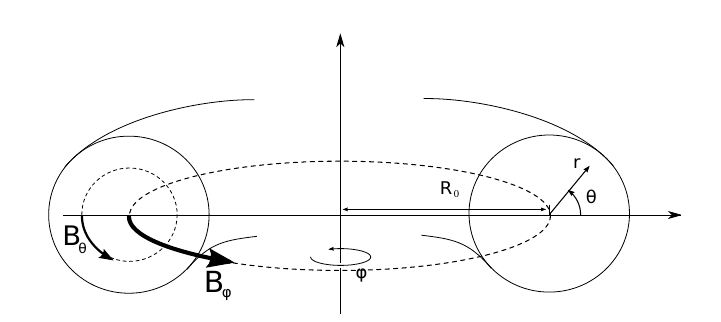
\includegraphics[width=8cm]{img/1_intro/toroidal_coords.png}
    \caption{Toroidal coordinates reference system}
    \label{fig:intro_toroidal_coords}
\end{figure}
\begin{itemize}
    \item $r = $ radial distance from central circular axis,
    \item $\vartheta = $ poloidal angle,
    \item $\varphi = $ toroidal angle.
\end{itemize}
Depending on their characteristics, the magnetic confined machines are divided in three principal categories:
\begin{itemize}
    \item \textit{Tokamak}, where both the toroidal and poloidal field components are present but with a net toroidal predominance that assumes essentially stabilization functions.
    \item \textit{RFP}, where the toroidal component is almost comparable to the poloidal to the extent that it reaches an inverted value at the boundary ( hence the name "\textit{reversed} field pinch"). Compared to the Tokamak configuration the stability of plasma is much more critical, but higher in efficiency.
    \item \textit{Stellarator}, where the geometry of the field is built by a complex displacement of non planar coils that encourage the winding of the plasma column.
\end{itemize}

\subsubsection{Tokamak configuration}
In the \textit{Tokamak} systems the toroidal field $B_\varphi$ is produced by a toroidal solenoid winded around the vacuum chamber, while the poloidal field $B_\vartheta$ is created by a strong toroidal current $I_p$ that flaws within the plasma. This current is in turn induced by means of solenoids coupled by the plasma ring (sometimes concatenated with a central coil). The same current is also used to heat the plasma by Joule effect ( Ohmic heating ) with a specific power of $P = \eta J^2$, defined $\eta$ as the plasma resistivity.
%
A fundamental parameter to define the \textit{Tokamak} typical features is $\beta$ defined as:
\begin{equation}
    \beta = \frac{<p>}{ \frac{B(a)^2}{2\mu_0} }
    \label{eq:magnetic_beta}
\end{equation}
with $<p>$ the average value of plasma pressure within a poloidal section. This parameter is the ratio between the mean kinetic pressure exerted by plasma, and the magnetic pressure of the field that is needed to confine it; the value assumed by $\beta$ is thus the measure of how effective the magnetic configuration results when seen as an energy balance.
If we compute the \eqref{eq:magnetic_beta} using the typical $B_\varphi$ and $B_\vartheta$ values that are present in a \textit{tokamak}, the resulting $\beta$ is about $2-3\%$; this means that the most of the spent energy that \textit{Tokamak} uses is not for the confinement but is is almost all used to stabilize perturbations.
Another key factor that defines the relative intensities of magnetic configuration is the so called "\textit{safety factor}" $q$:
\begin{equation}
    q(r) = \frac{rB_\varphi(r)}{R_0B_\vartheta(r)}
\end{equation}
As it will be widely described in the following sections, the radial profile of this parameter has a fundamental impact on the overall stability of the plasma: in more detail, a stable plasma configuration can be obtained by maintaining the $q(r)$ function strictly monotonic.
\begin{figure}
    \centering
    \subfigure[]{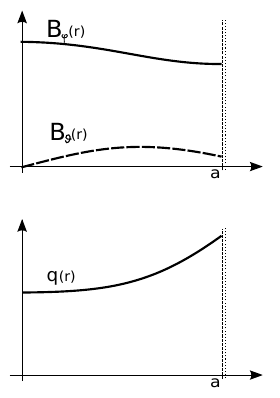
\includegraphics[height=5cm]{img/1_intro/tokamak_profiles.png} \label{fig:intro_safety_factor_profiles_a}}
    \subfigure[]{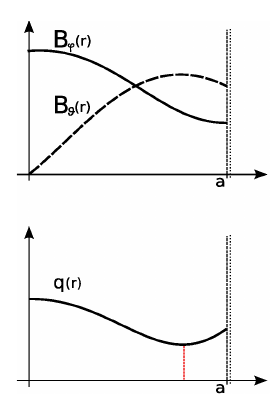
\includegraphics[height=5cm]{img/1_intro/rfp_profiles_norev.png} \label{fig:intro_safety_factor_profiles_b}}
    \subfigure[]{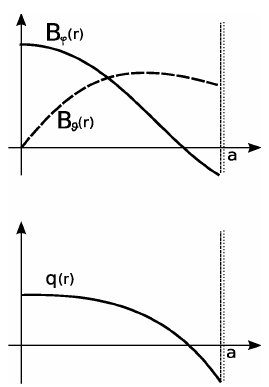
\includegraphics[height=5cm]{img/1_intro/rfp_profiles_rev.png} \label{fig:intro_safety_factor_profiles_c}}
    \caption{Magnetic field profiles for $B_\varphi$ and $B_\vartheta$, from the toroidal axis to the chamber boundary, for the toroidal confinement devices in \textit{Tokamak} configuration (a), \textit{RFP} without reversal (b), and \textit{RFP} with reversal (c)    }
    \label{fig:intro_safety_factor_profiles}
\end{figure}
As shown in \Figure{\ref{fig:intro_safety_factor_profiles_a}}, in the case of the \textit{Tokamak} configuration the monotonic property of the safety factor is guaranteed by an high ratio of $B_\varphi/B_\vartheta$. Still, because the poloidal fields is generated by the plasma current, to have such a high ratio of the fields it is necessary to maintain it under a certain threshold. This condition implies in effect a limitation for the possible Ohmic heating, bringing with it the need to find other means of additional heating, such as neutral particles injections (NBI), radio-frequency emissions resonating with cyclotron frequencies of electrons or ions, and so on.

\subsubsection{RFP configuration}
The \ac{RFP} is an axial-symmetric configuration provided with a toroidal current, similar to the \textit{Tokamak}. The difference between the two is in the ratio of the magnetic field components: while for the \textit{Tokamak} the toroidal field is of one order of magnitude over the poloidal, for the \textit{RFP} the two components are almost the same in average, and in the outer region the poloidal one tends to dominate. As a result, the most part of the magnetic field is generated from the plasma current itself, and with the same plasma current the total magnetic field that is exploited by \acs{RFP} is much lower that the one used by a \textit{Tokmak}. It can be also seen that, in the right conditions, once the plasma current has been induced, the toroidal field at the boundary inverts direction; this reversal gives a chance to obtain a monotonic factor $q(r)$ even with such low magnetic profiles. This is generally facilitated inverting the current direction on the coils of the toroidal system some instants after the pulse begins. For the \acs{RFP} model the profiles of $B_\varphi$(r), $B_\vartheta(r)$ and $q(r)$ are reported in \Figure{\ref{fig:intro_safety_factor_profiles_b}} and \Figure{\ref{fig:intro_safety_factor_profiles_c}} in the pre-reversal and reversal conditions.

Together with this reduced toroidal field intensity comes the possibility of reaching $\beta$ values much higher than those characterizing the \textit{Tokamak}. 
Given its magnetic topology, the RFP exploits the advantage of an easier technology involved in the electromagnetic system. This might be the case even for a reactor, where there might be no need for large superconducting magnetic coils; there is freedom in the choice of the aspect ratio and, in principle, ignition should be achievable with ohmic heating only.  
Although the high penalty payed by the \textit{RPF} is on the stability of perturbations that represents a profound limitation for the final achievable temperature, that remains one order of magnitude lower that the one promised by a \textit{Tokamak}.

% RW
A price to be paid for exploiting these advantages concerns magneto-hydrodynamic (MHD) stability. The safety factor q is in fact lower than 1 across the whole plasma, and negative at the edge. Figure 2(a) shows the q profiles of an RFP compared with those of tokamaks and stellarators. In the RFP q profile there are multiple resonant surfaces in the plasma, in particular for modes with poloidal mode numbers m = 0 and 1. This is shown in figure 2(b), which reports a typical RFP q profile. Two main kinds of global, current-driven MHD instabilities may be present in a RFP with resistive wall: (i) resistive kink/TMs, which are resonant in the plasma and are intrinsically linked to the sustainment of the configuration through the aforementioned self-organization process; (ii) RWMs, which are non-resonant ideal modes, slowed down by the resistive wall. RWMs in RFP are current driven and are present also at low plasma beta.


RFPs, however, can sustain very high plasma current and this makes it to be considered a potential fusion device with only Ohmic heating. On the other hand, the generation of plasma current needs a time variation of magnetic field which is sustained by the primary transformer. This time variation makes the devices, on some level, not in steady state. To overcome this problem, a toroidal configuration in which all the field components are generated by external coils is introduced. This device is the so-called stellarator. \Figure{\ref{fig:pinch_families}} shows a sketch of these two families. In the left graph, the red coils aligned toroidally are the toroidal field coils and the green helical ones are helical field coils. In the right graph, the red cylinder in the device center is the primary transformer. The red coils aligned toroidally are the toroidal field coils and the two green ones on the top and bottom of the device are the vertical stabilization coils. The stabilization coils are introduced because, due to the existence of Shafranov shift in toroidal devices, the plasma position needs to be optimized in order to avoid touches between the magnetic field and the first wall. 
The stellarator shows a much more complicated magnetic coil design than the one of the pinch family. Consequently, the manufacture process for magnetic coils are more complex for stellarators than for pinches. On the other hand, due to lack of plasma current, stellarators are almost free of disruptions.

Two dimensionless parameters are used to describe the RFP equilibrium. 
The pinch parameter \textbf{theta}, defined as:
\begin{equation}
    \Theta = \frac{B_\vartheta (a)}{ \left\langle B_\varphi \right\rangle }
\end{equation}
measuring how much the plasma and the magnetic field are pinched inside the torus; and the \textbf{reversal} parameter F, defined as:
\begin{equation}
    \mathrm{F} = \frac{B_\varphi(a)}{ \left\langle B_\varphi \right\rangle }
\end{equation}
that quantifies, instead, how much the toroidal field is \emph{reversed at the edge}.

The minimal model to compute the RFP equilibrium is the one-dimensional model governed by the MHD equilibrium equation $\nabla p = \Vec{j} \times \Vec{B}$ solved in cylindrical coordinates together with a parametric description of current and pressure profiles~\cite{Bonomo33}.
A more accurate model needs to add the toroidal geometry that produces outward radial displacement of magnetic flux surfaces, and hence a separation between the geometrical and the magnetic axis, i.e. the \textit{Grad-Shafranov shift}~\cite{freidberg2014ideal}. 
In this representation, RFP presents an axisymmetric equilibrium dependent on all toroidal coordinates $(r, \vartheta, \varphi)$  where the magnetic field lines are helixes. This RFP state (also called Single Helicity (SH) state that will be presented later on) can be described in terms of a helical Grad-Shafranov equation~\cite{Bonomo35, Bonomo36}, which represents the full 3D solution to the MHD equilibrium equation.


\section{RFX Experiment}
The first installations with $B_\varphi$ and $B_\vartheta$ fields of the same order of magnitude, i.e. the so called \textit{screw pinch} or stabilized \textit{zeta pinch}, started to operate at the beginning of the 60s; the most relevant was the ZETA\footnote{ZETA (Zero Energy Thermonuclear Assembly) that operated from 1954 to 1958 in Harwell (UK).}. At the time the results were considered mediocre: the machine presented a turbulent regime, followed by sporadic quiescent phases difficult to interpret. The first theoretical model was proposed by C.~B.~Taylor in 1974\cite{taylor}: He speculated, and proved afterwards, that the quiescent condition in ZETA corresponded to the spontaneous switch from the stabilized \textit{zeta pinch} system to the RFP by means of a self reversal of the toroidal field; and that this was also due to a minimum of the magnetic energy.

In the late 70s a research on such self phenomena started in Padova and brought to the making of RFX ( Reversed Field experiment ), a reversed field experiment machine with major radius $R_0 = 2m$ and minor radius $a = 0.5m$, that proved to be able to sustain a plasma current of $2MA$. In the period between 2001 and 2004 the same machine was modified to RFX-mod\footnote{in 1999 a severe damage of the plant was caused by a fire on the electrical source equipment. The experimental activity was not recovered until December 2004, after an intense rebuild of the plant and upgrade of the machine itself.} adding an active feedback control that widely improved its results.
\begin{figure}[ht!]
\centering
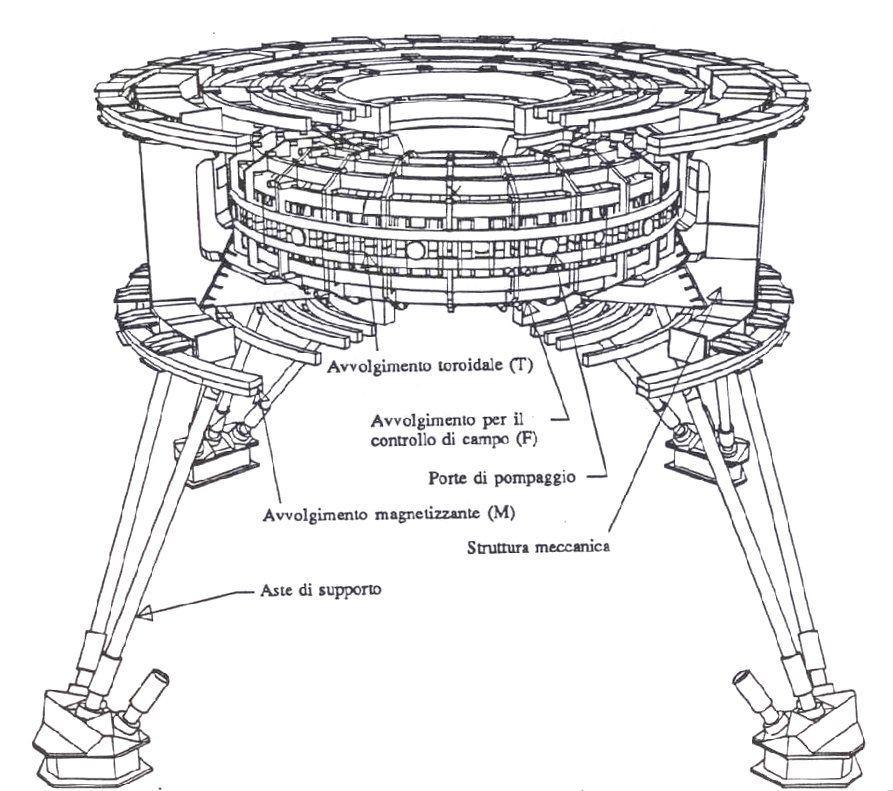
\includegraphics[width=0.5\textwidth]{img/rfx2}
\caption{ Perspective view of the RFX experiment }
\label{img:rfx}
\end{figure}
%
RFX is built of a vacuum vessel made of INCONEL~625\footnote{a nickel chromium molybdenum alloy that is frequently used to produce a stiff material with high temperature tolerance and good mechanical properties} and completely internally covered by 2016 carbon plates that shield it from sudden heat impulses generated by the plasma; it can resist to temperatures beyond 350C, and achieve ultra vacuum conditions $(P < 10^{-6} \text{mbar})$.
The structure, also called \textit{liner}, is composed by 72 cuneiform elements, shown in \Figure{\ref{fig:rfx_liner}} all displaced at 5 degrees one from the other in the toroidal direction, with an internal 1mm layer, an external 2mm, joint with a corrugated ring of 0.5~mm.
\begin{figure}[ht!]
\centering
\subfigure[]{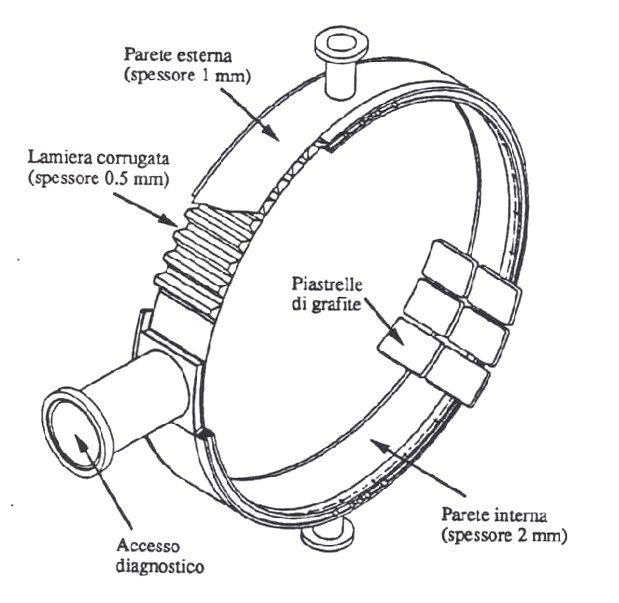
\includegraphics[width=0.4\textwidth]{img/rfx/liner_element.png} \label{fig:rfx_liner}}
\subfigure[]{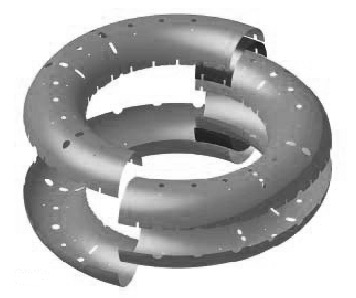
\includegraphics[width=0.4\textwidth]{img/rfx/shell.png} \label{fig:rfx_shell}}
\caption{ Perspective sketch of one of the 72 RFX vacuum chamber elements (a), RFX stabilizing shell components (b). }
\end{figure}


On the outer side the vacuum chamber is completely wrapped in a high conductive shell; the former choice was an aluminum foil, subsequently substituted by a chopper 3mm film in RFX-mod. The shell is composed by 4 parts of 180 degrees angular width on the poloidal direction, and a bit more on the toroidal one. Once the parts were assembled together, as shown in \Figure{\ref{fig:rfx_shell}}, two gaps remained unwelded: one on the toroidal direction and one in the poloidal direction in order to permit the magnetic fields to penetrate inside the shell\cite{th13}.

All currents, induced on the shell by radial field components (generated by a plasma perturbation), tend to counteract the plasma movement itself. This characteristic of the shell is able to stabilize fast perturbations\footnote{perturbations that happen in times in which the field remains stitched to the plasma (Alfv\'en theorem).} contributing to the horizontal equilibrium on the very initial states of the pulse~\cite{th19}. The value for a vertical field penetration time is about $\tau_w = 50 ms$\cite{th12}.


\section{Plasma control based on machine learning}

% supervised and unsupervised learning.
The very basic idea that defines the machine learning itself is to build a model that learns from experience. This happens it two ways: the model can be trained from a dataset that contains the true interpretation, or it can be trained without any information generating a representation of data itself. The two approaches are respectively called \textit{supervised} and \textit{unsupervised} learning.

Supervised learning is the task of learning to map input to output based on a set of previously known input-output pairs. It infers a function from labeled training data consisting of a set of training examples composed by pairs of input objects (typically vectors usually called features) and desired output values (called labels). The algorithm analyzes such data and produces an infer function, which can be then used for mapping new examples. In an optimal scenario this will allow to identify the class labels for unseen instances, because the learnt function will have generalized from training data to unseen situations.
The supervised learning are the most common and most used methods, because they provide a result with a direct meaning. 
This is well interpreted by neural networks that are actually one of the most simple approaches to machine learning, but at the same time one of the most promising, because they can very easily scale to tackle almost any kind of task with the same base units.
%
In principle the label information, i.e. the dataset ground truth that we use to "supervise" the model training, can be almost anything; we could choose to train a network to guess the whether forecast by counting the number of birds that fly by the yard. Any kind of data could be a useful argument if a weak relation could be extracted between data and labels.
From a statistical point of view, neural networks are nothing more than devices adapting to represent non-linear curves. 
Nevertheless, fitting a non linear curve is not a trivial task; the actual complexity of an interpolated model is of crucial importance. 
Indeed, while changing the complexity of the model, the best measure for the training data that the model can obtain becomes increasingly good, but the empirical fit performance first diminishes, then increases again. This happens because a model that is too complex starts to adapt to the training data and generalizes badly. In other words we could say that it learns how to represent the very training set, not any input data.
%
% course of dimensionality
The problem is the dimensionality of the input space. If the input feature vectors have very high dimension, the learning can be difficult even if the true function only depends on a small number of those features.  This is because the many "extra" dimensions tend to confuse the learning algorithm producing high variance on training. 
This problem is known in machine learning as the \textit{course of dimensionality}.
For this reason high dimensional inputs typically require the tuning of classifier to have low variance and high bias. In practice, if irrelevant features from the input data can be removed, this is likely to improve the accuracy of the learned function. 

A fusion experiment is very like to fall in this issue, because to acquire all the different aspects of the plasma characteristics a huge amount of diagnostics are required. A single kind of measure does not provide all the necessary information, and the actual glue that fixes the characterization of the machine has always been the physical model that subtends the phenomenon.
But this is not trivial as well: the data can be affected by many kind of noise and they may have only a partial access to the required variables that are needed for the physical model to run.

To solve this problem there are many algorithms for feature selection that seek to identify the relevant features and discard the irrelevant ones. 
Other methods require to apply preconditioning constraints that add existing relation among data: for instance, if we know that the data samples are ordered sequences, it makes sense to introduce algorithms that exploits this property such as the convolution.
This is an instance of the more general strategy of dimensionality reduction, that seeks to map the input data into a lower-dimensional space running the supervised learning algorithm or prior to it. 

A further possibility for the interpretation of high dimensional data could be their statistical representation.
This is the aim of the unsupervised learning, where similar algorithms are applied to feature without the aid of external information. The target this time is not to look for a given relation but for a representation of the data itself.
Several methods can be applied to achieve such dimensionality reduction: for example the principal component analysis, the singular values decomposition, and factor analysis among linear approaches; or the Autoencoders~\cite{Hinton504} as a neural network non-linear approach.

As stated, Autoencoders exploit the neural network architecture. They are built to have the same number of neurons both at the input and the output layers and the topology is organized to have an internal layer with less neurons to form a bottleneck. The training tries to match each data sample with the output by direct comparison.
The output values of the hidden smaller layer are then the reduced coordinates in the new space with a smaller dimension.
The overall path of the data through the network can be divided into two steps: a first net reduces the data dimensions \textit{encoding} the features in a small set of values, then a further net recovers the input data from the \textit{decoding} of the latent representation. 

Those values can be thought as the latent states of a non linear model representation and can be used to extract the new features that feed a supervised algorithm. In addition, a bayesian description of the latent variable can be applied, creating a true latent space. This is the case of the so called Variational Autoencoder (VAE) that is a \textit{generative} algorithm that recently gained a lot of attention.
In this case we create two distinct domains: the domain of the data and the latent one. On such models encoding a data can be seen as the inference to the latent space value, and decoding back to the data domain is referred as the \textit{generative} process. Hence the name of \textit{generative algorithms}.


% it is not the lose of the model
% - model can be applied to add information ( fourier for example )
% - model can be added to confront the dimensionality of the latent space

% no free launch theorem (perche neural networks)

% introduction to the bicycle example 
\subsubsection{How to ride the bicycle}

The primitive idea of the neural networks was originated by the first studies on brains, and inspired - but it is quite different in facts - by the internal organization of biological neurons. Similarly the intuitive idea of a non linear control system by means of deep generative networks is based on how the brain applies a wide sensory integration to perform complex ordinary tasks in an ”automatic” manner. 

A complex physical model, for instance, subtends the simple task of riding a bicycle. The engineering of the bike-rider system control can be quite articulated, many aspects being involved: the moments of inertia of the moving parts, the gyroscope effect of the wheel, the mechanical structural constraints and so on. 
Recently a formal description has been proposed~\cite{rideabike_nature_2016}~\cite{papadopulos_bike} proving a self stability of the bike that depends on the composition of the leaning and steering of the handlebar. Nevertheless conducting the bike along a curve or pass through obstacles requires a very tight control of movements, and no one actually apply any model for that. Learning to ride a bike is more related to fusing sensory data and shaping a space of equilibrium by means of small movements around the stability. A general map of all the acquired experience is progressively learnt by the brain that shapes a hidden state space representation of both the stimuli and the applied feedback. Doing that it generates a stable system where on any movement of the status we almost naturally associate an optimal reaction of bar steering and center of mass adjusting that permits to get the equilibrium back.
The point of this digression is that we are not really learning how to control a bike from classifying events - such as: I stayed up or I felt - but from the shape of the reduced space that represents sensors and actions. In the world of machine learning this translates in the unsupervised approach to represent the system status over (or beside) the training on supervised observations, and this kind of control in such complex systems turns to be more effective and robust than applying a physical model.

Back to the case of a fusion experiment, this kind of control could exploit the scaling properties of neural networks to implement an unsupervised training of acquired data. This can collate all the important aspects of the plasma properties, representing them in a reduced state space. At this point a simple linear controller could be applied to set the dynamic behavior of the system, or a further non-linear dynamical representation could be also done by means of \acl{RNN}.
%to constrain the system dynamics by plotting boundaries around the latent space equilibrium.

Once applied to many diagnostics, a cascade of encoders, from the raw signals on the machine up to the control loop, could effectively ease the problem of dimensionality and create a map that extracts the important features from the physics of plasma. Moreover, in this hierarchy a set of feedback signals of the system status could also meant to be fed back in the early sensors encoders. In such way even the feature extraction could be \textit{conditioned} on the state of the machine, and the data extracted could be optimized by the training process itself.

However to ensure a responsive feedback control for the experiment, these models must be operated in real-time.
The beauty of a neural network structure come to help again: attempting a quantization of neurons activation functions, such models can be modified to be converted to embedded firmware. Those firmware, approximating the deep generative model to a set of simple operations, fit well with the simple logic units that are largely abundant in FPGAs. This is the key factor that permits the use of affordable hardware with complex deep neural topology and operates them in real-time. 

But this still remain a very complex set of algorithms and hardware that must be properly adapted to the application specifics and fitted into a renewed acquisition chain.
To this purpose we started the development of a framework, named Mildstone, that aims at organizing the entire process of creating new "smart" devices for data acquisition that implement the presented models but also fit in the chain of acquisition (i.e. provide the data storage, the signal conditioning and so forth).
This is not a new software per se, but adopts many consolidated tools. Among them: Tensorflow for machine learning, MDSplus for data acquisition, MARTe for run-time process and Vivado for FPGA development.

Some points remain open though, one above the others is the fact that with the current technology the network must be trained \textit{off-line} the run of experiment. This could appear not to be such a limitation, but it turns to prevent the possibility of learning the control from the applied variational. If in the future the network quantizers will be able to retain some flexibility in an \textit{on-line} changing of the network weights, a possible self training of the network could be adopted, giving a chance for the experiment to really learn the control.


\section{Structure of the document}
In Chapter 2 a brief description of the plasma single fluid equilibrium is presented as an introduction to tearing perturbations and the quasi single helicity state of the plasma. 
In Chapter 3 some basics of machine learning are defined with a particular attention to the neural network regression and to the principles of regularization. 
Chapter 4 discusses a possible control scenario based on machine learning, and a possible redefinition of the acquisition chain obtained by the use of FPGA equipped "smart" sensors.
Chapter 5 presents Mildstone as a possible set of tools to organize all the steps that are required to define this kind of "smart" sensors.
In Chapter 6 and Chapter 7 a Variational Autoencoder is used to represent the plasma temperature profile as it has been acquired by RFX-mod Soft X-Ray diagnostic. The resulting embedded space is further used to try a mapping from magnetic sensors and from some plasma parameters to guess the temperature.
In Chapter 8, in addition to our conclusions, a technique to extract information from learnt hidden "factors" is described, and some possible future enhancements are discussed.

\chapter{RFP Equilibrium}
\label{section:2_equilibrium}

The success of magnetic confinement systems depends on the ability to maintain the plasma in equilibrium in the presence of small perturbations
that could compromise its stability. In Tokamak and RFP type experiments, the instabilities that produce macroscopic effects are described, in their simplest form, by the plasma fluid model MHD ( magnetohydrodynamic model ). 
We abandon the kinetic description of the single particle to consider the set of charges, thinking of the plasma as a fluid: the dimensions of the survey region are much greater than the Debye length and the Larmor radius. Therefore, a discrete system with separate charges is no longer observed.


%  __  __ _   _ ____  
% |  \/  | | | |  _ \ 
% | |\/| | |_| | | | |
% | |  | |  _  | |_| |
% |_|  |_|_| |_|____/ 


\section{Single fluid magnetohydrodynamic equilibrium}

In the MHD model the equations of classical electromagnetism are combined with those of the fluid motion. Typically the analysis of fluid plasma involves the generalized movements of each ionic species; however, for simplicity it is possible to consider each pair of values relating to ions and electrons in a single parameter and thus obtain a single fluid trend. Moreover, remembering that for fusion gases there is almost neutral charge $n_i = n_e$ the charge density term $\rho = e(n_i - n_e)$ can be omitted. The relevant quantities are thus:
\begin{itemize}
    \item the mass density of the fluid
    \begin{equation}
        \rho_m = n_e m_e + n_i m_i
    \end{equation}
    \item the mean current density per unit volume
    \begin{equation}
        \mean{J} = e(n_i \mean{v_i} - n_e \mean{v_e})
    \end{equation}
    \item the fluid pressure
    \begin{equation}
        p \approx n_e k T_e + n_i k T_i
    \end{equation}
\end{itemize}
With this variables the fluid equations and the conservation of moment and mass can be defined:
\begin{align}
    \pdv{\rho_m}{t} + \nabla \cdot (\rho_m \Vec{v}) &= 0 \\
    \rho_m \left( \pdv{\Vec{v}}{t} + \Vec{v} \cdot \nabla \Vec{v} \right) &= \Vec{J} \times \Vec{B} - \nabla p
    \label{eq:mhd_momentum} 
 \end{align}
where the electromagnetic interaction can be added with the Maxwell and Ohm relations:
\begin{align}
    \nabla \times \Vec{E} &= - \pdv{\Vec{B}}{t} \label{eq:faraday} \\
    \nabla \times \Vec{B} &= \mu_0 \Vec{J} \label{eq:ampere} \\
    \nabla \cdot \Vec{B}  &= 0 \\
    \nabla \cdot \Vec{E}  &= 0 \\
    \Vec{E} + \Vec{v} \times \Vec{B} &= \eta \Vec{J} \label{eq:ohm}
\end{align}
Finally to close the system you can choose to introduce alternatively:
\begin{itemize}
    \item the perfect conductivity of the plasma to obtain the cancellation of the resistivity\footnote{In fact the resistivity is a term related to the plasma temperature through the Spitzer relation \begin{equation}
        \eta = 5 \times 10^{-5} \frac{Z \log(\Delta)}{T_e^{3/2}}
    \end{equation}} term in \eqref{eq:ohm}
    \begin{equation}
        \eta = 0
    \end{equation}
    \item the addition of a state constraint for the ideal gas, considering only isothermal or adiabatic transformations:
    \begin{equation}
        \pdv{}{t}\left( \frac{p}{\rho_m^\gamma} \right) = 0
    \end{equation}
    \begin{align}
        \gamma &= 1    \hspace{3cm} & \text{isotherms} \\
        \gamma &= 5/3  \hspace{3cm} & \text{adiabatic}
    \end{align}
\end{itemize}
From the MHD equations it is also possible to derive some considerations regarding the movement of the plasma: for example, combining the Ampere equation \ref{eq:ampere} with that of Ohm \ref{eq:ohm} we obtain the variation of the induction field, which turns out to be the composition of a flow term and a field diffusion term.
\begin{equation}
    \pdv{\Vec{B}}{t} = \nabla \times ( \Vec{v} \times \Vec{B} ) + \frac{\eta}{\mu_0} \nabla^2 \Vec{B}
    \label{eq:coupling_plasma_1}
\end{equation}
This term describes the dynamic coupling between the magnetic field and the displacement of the fluid. If we compare the two contributions of \eqref{eq:coupling_plasma_1}, considering as viscosity factor $\nu_m = \eta/\mu_0$, we get:
\begin{equation}
    \frac{|\nabla \times \Vec{v} \times \Vec{B}|}{|\nu_m \nabla^2 \Vec{B}|} \simeq \frac{\frac{x \cdot B}{L}}{\nu_m\frac{B}{L^2}} = \frac{vL}{\nu_m} \equiv \mathcal{R}_m
\end{equation}
where L is the characteristic variation length for the quantities considered. $R_m$ is called Magnetic Reynolds Number and quantifies the prevalence of plasma flow phenomena with respect to $\Vec{B}$ diffusion.

When, as generally happens, it is the first component to be dominant $(R_m >> 1)$, the relationship expresses the conservation of the magnetic flux through any surface bounded by a closed line, independently of the movement of the fluid. This result is also expressed by Alfven's theorem: in a conductive fluid with zero (or very small) resistivity, the magnetic field lines remain frozen in a given volume of the fluid itself.
In conclusion it can be said that a plasma of small magnetic viscosity can be more effectively compressed by strong gradients; at the same time, however, a turbulent motion is obtained in which the variation of the field increasingly depends on transport phenomena.




\subsection{Static equilibrium}
The study of the plasma MHD instability mainly concerns the perturbations of the ideal system starting from a magneto-static equilibrium point. In this state the relationships that present a temporal variation are null, thus, imposing $\eta=0$ and $\pdv{}{t} = 0$ the system become:
\begin{align}
    & \nabla \cdot \Vec{B} = 0 \\
    & \nabla \times \Vec{B} = \mu_0 \Vec{J} \\
    & -\nabla p + \Vec{J} \times \Vec{B} = 0
\end{align}
% \begin{equation}
% \systeme*{
%     \nabla \cdot \Vec{B} = 0,
%     \nabla \times \Vec{B} = \mu_0 \Vec{J},
%     -\nabla p + \Vec{J} \times \Vec{B} = 0
% }
% \end{equation}
From the third equation it is clear that the pressure gradient is maintained orthogonal to the field and current lines, constructing a set of nested surfaces, called magnetic flux surfaces\footnote{It should be noted that the magnetic and current fields of the first and second relations are solenoidal and lead to necessarily closed surfaces. If we consider a constant pressure module along this surface, with an intersection angle between the perpendicular field vectors everywhere, we obtain the torus as a possible solution.}. These are said rational surfaces when the field lines that run through them recombine on themselves after a few toroidal turns, or ergodic when, not recombining, they cover the entire surface.

The effects of a generic stability disturbance of the balance just described is now made explicit using the spatial transformation in Fourier series; the perturbation $\Tilde{\psi}$ can be expressed as:
\begin{equation}
    \Tilde{\psi}(\Vec{r},t) = \sum_k \Tilde{\psi}_k(r) e^{i(\Vec{k}\cdot\Vec{r}-\omega t)} = \sum_k \Tilde{\psi}_k e^{i(m\vartheta+n\varphi-\omega t)}
\end{equation}
where $\Vec{r} = (r,\vartheta,\varphi)$ is the displacement vector in toroidal coordinates, and $\Vec{k}$ is the vector of the respective wave numbers.

Its frequency is the expression of the transform in time, and it is in general a complex value $\omega = \omega_R + i \omega_I$, in which the real part expresses the propagation speed of the wave, and the imaginary part represents the growth, damped $(\omega_I < 0)$ or exponential $(\omega_I > 0)$, of the amplitude of the perturbation. The step of this perturbation is therefore obtained by $(m\vartheta + n\varphi = \text{const})$, that is:
$$  m d\vartheta - n d\varphi = 0    $$
$$  p_p = \int_0^{\Delta\varphi} d\varphi = \int_0^{2\pi} \frac{m}{n}d\vartheta = \frac{m}{n} 2\pi  $$
In the same way the step for the field lines is:
$$  \frac{R_0 d\varphi}{r d\vartheta} = \frac{B_\varphi}{B_\vartheta} $$
$$  p_b(r) = R_0\Delta\varphi = \int_0^{2\pi} \frac{1}{R_0} \frac{B_\varphi(r)}{B_\vartheta(r)} r d\vartheta = 2\pi r \frac{B_\varphi(r)}{B_\vartheta(r)}  $$

\begin{equation}
    p_b(r) = p_p    \hspace{2cm} 	\iff \hspace{2cm}  q(r)\equiv \frac{r}{R_0}\frac{B_\varphi(r)}{B_\vartheta(r)}=\frac{m}{n}
\end{equation}



The perturbation $\tilde{\psi}(m,n)$ whose steps are coupled with the field lines is called \textit{resonant}, and is the cause of instability. In this picture it is evident that the \emph{''safety factor''} $q(r)$ is related to the stability of the plasma; in fact when $q$ is rational, any displacement of the plasma from the equilibrium position can have a component that is screwed onto the magnetic surfaces with the same periodicity as the field. If, on the other hand, $q(r)$ is irrational the field lines continue to be screwed onto the toroidal surface without ever rejoining with themselves, sweeping ergodically the entire surface.


%%%%%%%%%%%%%%%%%%%%%%%%%%%%%FIGURA%%%%%%%%%%%%%%%%%%%%%%%%%%%%%%%%%%%%%
\begin{figure}[ht!]
 \centering
 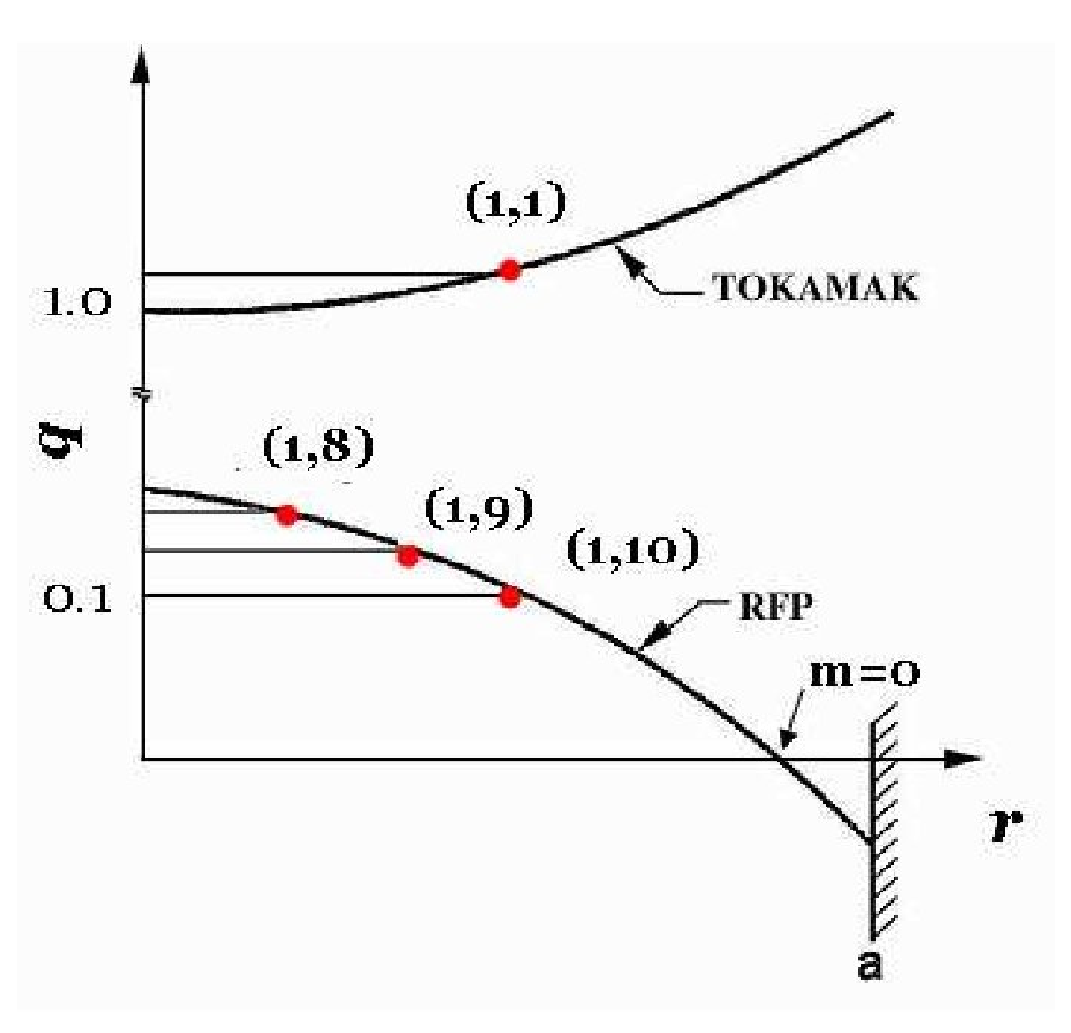
\includegraphics[ width=8cm ] {img/2_eq/safety-tokarfp.eps}
 \caption{Comparison of $q$ profiles, with respect to the position of the torus axis; for Tokamak and RFP type machines. }
 \label{fig:profiles-tokarfp}
\end{figure}
%%%%%%%%%%%%%%%%%%%%%%%%%%%%%%%%%%%%%%%%%%%%%%%%%%%%%%%%%%%%%%%%%%%%%%

In turn, more adjacent surfaces that have the same safety factor couple with each other giving rise to resonance phenomena, becoming themselves a source of instability; for this reason we introduce the parameter called \emph{'' shear ''}
%
\begin{equation}
 s(r) \equiv \frac{r}{q(r)}\frac{dq(r)}{dr} = \frac{r}{p_b}\frac{dp_b}{dr}
\end{equation}
%
which represents the variation along $r$ of the pitch of the field lines. It is therefore essential that the pitch is variable monotonically to avoid destabilizing the entire system.
In \Figure{\ref{fig:profiles-tokarfp}} the radial profiles of the safety factor for Tokamak and RFP experiments are plotted; note that the configuration has been chosen in such a way that the trends represent strictly monotone functions.

\subsubsection{The cylindrical approximation}

Although the real machine has a toroidal shape, to simplify the treatment of the forces involved in the MHD model it is considered a cylindrical approximation, ideally imposing also the quantities along the longitudinal axis of the cylinder periodic. In this particular geometry, which will also be used for the study model subject of the present discussion, it is easier to identify the two current configurations that realize the  \emph{''pinch''} effect (striction) of the plasma \cite{fridberg}\cite{ortolani}, called $theta$-\emph{pinch} and $zeta$-\emph{pinch}\footnote{currents along the angular and axial direction of the cylinder, transformations of the poloidal and toroidal coordinates respectively.}.

For example, inserting the Ampere equation \eqref{eq:ampere} into the Navier-Stokes \eqref{eq:mhd_momentum} of the continuity of the momentum, we obtain a relation that describes the behavior of the pressure in the plasma:
\begin{equation}
 \label{eq:mhd_sol1}
 -\nabla \left( p+\frac{B^2}{2\mu_0} \right) + \frac{
  (\Vec{B}\cdot\nabla)B}{\mu_0} = 0
\end{equation}
Still remaining in the steady state of equilibrium, where the term of time derivative is null, the \eqref{eq:mhd_sol1} describes the equilibrium that is established between the pressures, kinetic and magnetic, and the effect of the curvature of the ${B}$ field lines (so-called magnetic tension). If we consider, then, a simple example of linear pinch, in which the magnetic tension component also disappears, the magnetic tension is in fact an expression of the curvature of the field lines, we can see how the striction effect depends on the gradient of field of the plasma column. Thus it is possible to reformulate the parameter $ \beta $ which for the linear pinch depends precisely on the relationship between the external field and the field penetrated into the plasma:
\begin{equation}
\beta = \frac{p}{p_{mag}} = 1-\frac{B_{int}}{B_{ext}}
\end{equation}



\subsection{Classification of instabilities}
\label{sez:classificazione}

The general classification of plasma instabilities is usually based either by their main physical causes, or the place where they rise up.
%
In the former case we divide them by the source of destabilization, there can be instabilities: pressure driven, current driven or particle driven. 
The pressure driven modes, also called “pressure driven instabilities” ( for example “interchaged modes or balooning modes” are pressure driven), can be derived directly from the equilibrium equation (force balance between kinetic and magnetic pressure) when we have strong gradient in the perpendicular current.
The current driven modes are instabilities that grow in time, they dissipate energy. In this case the parallel current gradient is the main driving phoenomena: kink modes are an example of current driven instabilities. Kink modes can be either internal or external; and usually the external kink sets the actual limit on the maximum achievable current. So the q factor at the edge instability is set by an external kink. Certainly they can also combine and give rise to a balooning-kink mode.

Another classification criterion for the instabilities is based on the place where they rise; the modes can be: \emph{external} when the edge boundary involved or \emph{internal} when it develops only inside plasma. 
They are also called \emph{fixed-boundary} and \emph{free boundary} instabilities when identified with respect to the column surface displacement. The former have an effect inside the column, not affecting the movements of the plasma surface, the latter \emph{free boundary} instabilities are macroscopic and involve the overall displacement of the vacuum-plasma interface.
This is the worst case because they usually lead to overall confinement loss: if such an instability develops, the distorted shape leads to an excess of heating flux on the plasma facing components. The parallel flux of energetic particles from the plasma toward the facing component, sputters and/or evaporates the material, polluting the plasma with high-Z atoms causing  radiative losses (the \emph{thermal quench}) which finally abrupt end of the discharge (the \emph{current quench}).

Any mode can be further labelled by the wave numbers that describe its relative perturbation
with the pair of values $(m, n)$:
$\tilde{\psi}(\Vec{r}) =
\Tilde{\psi}_0(r)e^{i(m\vartheta+n\varphi)}$.

The modes with poloidal number $m = 0$, (i.e. $(0,n)$) give rise to the \emph{``sausage instabilities ''}. These instabilities can be easily described by observing a pure z-\textit{pinch} experiment in cylindrical geometry: as shown in the \Figure{\ref{fig:press-curr1}}, the axial constrictions of the plasma column involve different values of $B_\theta \sim 1/r$. The kinetic pressure is the same everywhere, while the magnetic pressure tends to be stronger at the saddle, giving rise to bulges that are increasingly amplified.
%
\begin{figure}[ht]
 \centering
 \subfigure[]{ \label{fig:press-curr1}
 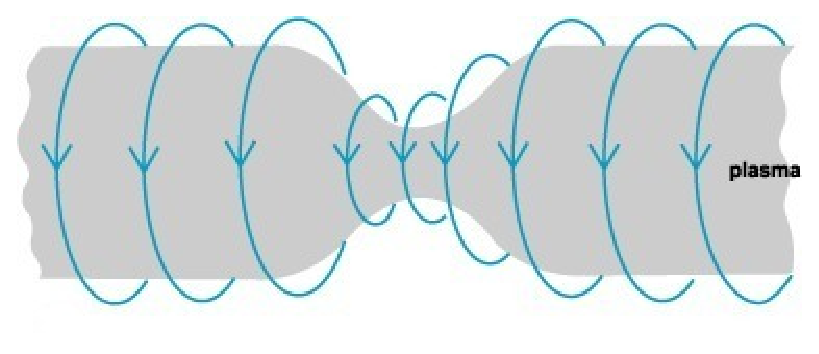
\includegraphics[ width=5cm ] {img/2_eq/press-curr1.eps}}
 \subfigure[]{ \label{fig:press-curr2}
 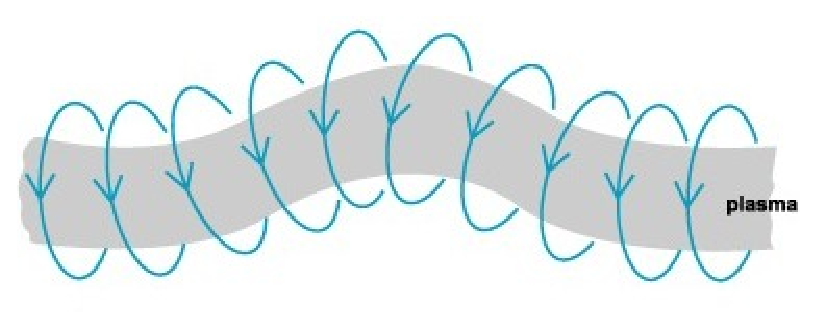
\includegraphics[ width=5cm ] {img/2_eq/press-curr2.eps}}
 \caption{Pressure (\emph{sausage}) and current (\emph{kink}) instabilities}
\end{figure}

The modes with poloidal number $m = 1$ (i.e. $(1,n)$) from another class of instabilities called \emph{``kink''}, \Figure{\ref{fig:press-curr2}}. In this case the curvature of the column of plasma involves the thickening of the field at the lower surface concave part; there is again an increase in the magnetic pressure which gradually amplifies itself.
%
These instabilities are generally the most unstable and dangerous, as they rapidly grow and so is hard to get rid of them, with growth times in the order of $1/\tau_A$ \footnote{$\tau_A = a/v_A$, with $ v_A $ the Alfvén speed and $a$ the minor torus radius, it refers to field variations frozen plasma \cite{fridberg}.}; they are seeded by the resonant surfaces and are generally stabilized by a strong toroidal field.

As a conclusion, recalling the considerations made in the previous paragraph about the safety factor $ q $ and the shear, it is interesting to mention now the the Kruskal-Shafranov criterion for stability in tokamak configurations. Kink modes $(1,n)$ we have resonance at $q(r)=1/n$; to ensure stability it is necessary to keep $q>1$ everywhere inside the plasma. On tokamaks $ q (r) $ has usually a minimum in the center of the column and then increases towards the periphery; therefore, since the criterion has to hold everywhere, the value of $q$ on the periphery should remains bounded at $ q(a) \gtrsim 3 $\footnote{Therefore placing the value at the periphery of $q(a)=\frac{a}{R_0}\frac{B_\varphi(a)}{B_\vartheta(a)}~\simeq~3$ and considering a typical aspect ratio $a/R_0 \simeq 3$, this criterion explains the strong amplitude difference between the toroidal $B_\varphi$ and poloidal $B_\vartheta$ fields of the tokamak.}.


\subsection{The resistive wall modes}

An important example of kink instability is represented by the so called \ac{RWM}. They are the remnant of the ideal kink modes when the plasma is cased in a continuous conductor of finite resistance (the \emph{shell}). They are relatively slow, since they depend on the characteristic resistive decay time of the shell (usually made of metal), which translates in the penetration time of the field: $\gamma_{RWM} \propto 1/\tau_w$. Their value is defined as:
%
\begin{equation}
 \tau_w = \mu_0 \sigma r_w \delta_w
\end{equation}
%
where $\sigma$ is the conductivity of the wall, $ r_w $ the corresponding radius and $\delta_w \ll r_w$ the wall thickness. 

The \acs{RWM}s are characterized by the presence of a radial field $b_r|_{r=r_s} \neq 0$, where $ r_s $ is the radius of the resonant surface that generates the unstable mode, which makes the recombination of the field lines possible.

A spontaneous growth of \acs{RWM} instability has been experimentally observed in \acs{RFP} with non-resonant \emph{'' current driven ''} perturbations characterized by $ m = 1 $, and several harmonics $ n $ which can be simultaneously unstable with different growth factors $\gamma$\cite{pizz46}\cite{pizz47}\cite{gregoratto}.

In tokamak configuration the spectrum of RWM modes is usually characterized by the dominant toroidal component of mode $ n = 1 $ and by various poloidal modal components with $m=2,3,4$ $(2,1),(3,1),... $ etc.
\footnote{
However, recent experiments shown that in some tokamak configurations there is the presence of ideal \textit{kink} instabilities of non-resonant \emph{current driven} modes. These instabilities seem to be excited by the free energy in the gradients of the plasma current that arise during the ascent current ramp~\cite{baruzzo9, baruzzo10, baruzzo11}. This effect has the double disadvantage of limiting the maximum growth rate obtainable for the induction of the plasma current and, at the same time, they define a minimum value of the safety factor at the edge.}.
%
Usually the study of \acs{RWM}s is conducted in \acs{RFP} configuration, because in this context they are more easily reproducible and do not cause great damage to the walls of the chamber. Nevertheless, their stabilization is an important challenge also for modern Tokamak machines, being one of the main factors that limit the high $\beta$ configurations.

To control the wall modes, in recent years some stabilization methods applicable to both the two configurations have been studied. Among these the stabilization based on the plasma rotation effect consists in the production of a toroidal angular momentum through the orientation of the neutral beam injector. This theory suggests that stabilization can be effectively achieved for angular velocities above a critical value ($\Omega_c \approx 1 kHz$) However, experimental observations have shown that, although this value is sufficient to maintain stability, in fact it is not compatible with values of $\beta$ above a certain threshold \cite{baruzzo12}. In fact, beyond a given restriction, the plasma tends to slow down the rotation, creating the conditions for the onset of \acs{RWM}. This method is effective for ensuring the functioning of recent Tokamak configurations~\cite{baruzzo12}, but not for the acs{RFP} configuration~\cite{baruzzo13}; it is also not yet clear whether it can be successfully used in the ITER project\footnote{International Thermonuclear Experimental Reactor, in Latin `` the way '': it is the machine that represents the passage between the studies performed so far on the physical and technological aspects of the fusion and the future power plant for the production of fusion energy.} due to the limited torque actually applicable by high-energy \acs{NBI}.
%
So, the solution offered by the presence of the conductive shell in the ideal wall hypothesis (perfectly conductive and continuous) has proved to be able to maintain stable equilibrium in presence of high growth factor MHD perturbations~\cite{gimblett_5,gimblett_6}; in the real case where the wall has a minimal - but not null - resistivity, the system generates \acs{RWM} type instabilities.

As already anticipated, the RFX experiment was modified with the introduction, among other innovations, of a sophisticated system of active control of the MHD modes. It consists of 192 \textit{saddle coils}: 48 poloidal arrays with 4 coils each, separately fed and located on the outer surface of the shell at a distance of $r_c = 0.5815m$. The corresponding magnetic sensors, capable of detecting the radial and toroidal field, are positioned inside the conductive wall at a distance of $r_s = 0.508m$. The control aims to counterbalance the radial field components generated by the unstable perturbations of the RWM modes. Indeed, the amplifier system is able to generate non-axisymmetric modes and can operate configured in different ways: for example the so called \emph{'' Virtual Shell ''} (VS) is a local feedback system that, while not taking account of the global effects on the plasma, is already able to strongly reduce the radial field component $b_r$\cite{pizz78}\cite{pizz79}. Other methods has been studied as well. Some propose the description of the wall crossing analyzing the aliasing components introduced by the actuators in the higher harmonics\cite{pizz81}.

%% RFP
% - Taylor relaxed state (need of reversal) -> magnetic shear
% - reversal can not be produced by coils ... plasma is needed
% - no need for superconducting coils and no current limit  -we don't satisfy Kruskal-Shafranov (safety factor)-
%   (10MA target to have a good condition in terms of neutrons production) -> ohmic heating is possible.
% - In RFX-mod the ohmic heating power can scale up to 60MW of coupled power (that is a huge amount of power)
%   in a stellarator to reach the same power deposition using external heating you need very high power.
% - High current possibility means -> High particle density limit ... Greenwald limit

% - why High plasma current? because 


\subsection{RFP Dynamo effect}

The ideal MHD is a plasma approximation with resistivity set to zero: this has the key direct consequence that the Alfven theorem holds. This states that the magnetic flux can be seen as ``\textit{frozen}'' inside the plasma (or in the other way around the plasma is frozen with the magnetic field line).
This approximation can be applied on experimental conditions where the resistivity is small and can be negletcted. Since in the plasma resistivity inversely depends on the temperature, this usually corresponds to high temeprature regimes.
The direct consequence of the ideal conditions on plasma structure topology is that it does not change ans maintains the nested closed flux surfaces; on the other hand, if plasma is thought to be resistive, the magnetic field topology is allowed to change, and in some cases yielding field lines or flux surfaces to be cut and recombined, a process called \textit{magnetic reconnection}. The regions where the currents can flow are called the current sheets while the reconnected flux regions are the \textit{magnetic islands}. The plasma changes in its defined topology, and it is usually undesirable because within the magnetic islands the quality of confinement is decreased; however in certain conditions this is a good outcome for RFP as it will be shown in few lines.

What has been shown so far is that, even if in the ideal condition the plasma has been made stable through a suitable shaped safety profile, other instabilities can rise through resistive components in the MHD equation the field lines tear and reconnect each other in the so called \textit{magnetic islands}.
In an RFP system the plasma resistivity cannot be neglected and there is a need for a mechanism to maintain the magnetic configuration balance over time, against the magnetic diffusivity which tend to flatten out the toroidal field.

The description of this process can be made clear by approximating the plasma column to a cylindrical conductor and using equations given in~\eqref{eq:mhd_sol1} the magnetic field in such a condition is subject to a resistive diffusion phenomenon described by:
\begin{equation}
    \pdv{\Vec{B}}{t} = \frac{\eta}{\mu_0} \nabla^2 \Vec{B}
\end{equation}
Resolving the differential equation this field component - that describes the equivalent toroidal component in RFP - presents a decay time constant of $$\tau_R = \mu_0 a^2 / \eta$$ 
where $\eta$ being the resistivity of the equivalent conductor and $a$ its radius.
On the contrary the experience shows that the RFP configuration is maintained for indefinite times, much longer than $\tau_R$. This is the result of a spontaneous mechanism of regeneration of the dissipated magnetic toroidal flow, called \textit{dynamo} in analogy with similar phenomena in astrophysical and geophysical plasmas. The dynamo mechanisms are responsible for generating an electric field which is added to the externally applied one and helps to drive the missing current density. 
It is clear to see that at the reversal point, the value of the poloidal current $J_\vartheta$ is not zero. The induction equation and Ohm’s law:
\begin{equation*}
    \pdv{\Vec{B}}{t} = - \nabla \times \Vec{E}  \hspace{3cm} \Vec{E} + \Vec{v} \times \Vec{B} = \eta \Vec{J}
    \label{eq:ohm_dynamo}
\end{equation*}
At the reversal location $E_\vartheta = 0$, 
but $J_\vartheta \neq 0$ in agreement with the typical RFP discharge profile shown  in~\Figure{\ref{fig:intro_safety_factor_profiles}}.
The reversal profile is then not generated by $d\Vec{B}/dt$, which is null in stationary condition, but must be due to am internal \textit{dynamo} mechanism, linked to the flow term $\Vec{v} \times \Vec{B}$.

This poloidal component $J_\vartheta$ is then responsible for the regeneration of a toroidal field in the core and for the sustainment of its reversal at the edge. It is worth noting that in \eqref{eq:ohm_dynamo} there is no need of many modes concurring to the dynamo, and the whole mechanism can be carried by a single perturbation~\cite{Bonomo39}.

The time evolution of a magnetic island is described by the Rutherford equation and it is related to:
\begin{equation}
    \frac{\tau_R}{r^2} \frac{dw}{dt} = \Delta^\prime
\end{equation}
%
where $\tau_R$ is the local resistive time, $R$ is the geometrical radius, $w$ is the reconnected island width, and $\Delta^\prime$ is the logarithmic jump of the radial magnetic field component across the rational surface.
%
The value of $\Delta^\prime$ is than related to the radial magnetic field in the jump:
\begin{equation}
    \Delta^\prime (w) = \frac{1}{B_r} \left( \frac{dB_r}{dr}_\text{left} - \frac{dB_r}{dr}_\text{right} \right)
\end{equation}
%	
This jump correspond to a thin layer of finite current on the resonant surface and defines the \emph{classical tearing mode} which is a current driven instability.

\subsection{SH and QSH states}

The RFP configuration depends on plasma current that is externally driven by an applied toroidal electric field $E_\varphi$. 
The power dissipation through the plasma finite resistance (aka. Ohmic heating), together with the striction applied by magnetic pressure ($\beta$), heats the plasma and produces peaked electron temperature profiles. 

But the plasma resistivity $\eta$ inversely depends on electron temperature\footnote{the complete relation has been formulated by Spitzer as: $$\eta_\bot  = \frac{4\sqrt{2\pi}}{3} \frac{Z_e^2 m_e^{1/2} \ln{\Delta}}{(4\pi\epsilon_0)^2(k_B T_e)^{3/2}} $$.}
as: $(\eta \propto \frac{1}{T_e^{3/2}})$, so to a local increase in electron temperature corresponds a decrease in resistivity, and hence to a further rising of the current density in that region, and obviously a related increase of Ohmic deposition. In this way, steep localized gradients of the current density profile tend to be generated, in which there is enough free-energy to drive an unstable spread spectrum of tearing modes $(m = 1, |n| \geq 2R_0 /a)$. The non-linear interaction of the $(m = 1, n)$ perturbations has been both theoretically explained and proved by experiments to be responsible of $(m = 0, n \geq 1)$ modes generation, which are resonant at the reversal surface \cite{Bonomo33}. This high magnetic activity translates into a populated spectrum of m = 0 and m = 1 modes.
Because of the many m=1 modes active in the spectrum, this RFP regime is also called \acl{MH}.

These generated tearing modes play an important role in the previously mentioned \textit{dynamo} effect; is worth noting though that, as already stated, the MH regime is not the unique solution to it. 
In fact, spontaneous helical symmetric states called \acl{QSH}, in which a single mode dominate the m = 1 spectrum, have been measured in all existing RFP machines~\cite{Martin_1999}; an example of such a spectrum is shown in~\Figure{\ref{img:MHQSH_b}}. The QSH state is not yet completely understood and is considered as an experimental evidence; however a theoretical approach for a possible Single Helicity (SH) RFP equilibrium, in which only one m = 1 mode is present, has been conjectured~\cite{Cappello_1996}. QSH is actually not a pure SH, since there is a residual background of modes with $m = 1, |n| > n0$ where $n_0$ being the dominant; thus these modes are usually referred as the “secondaries”. In addition in high current regimes we also experience very rapidly switching between MH to QSH states. This gave reason to define a new magnetic parameter to highlight the state, that is the \textit{ratio of dominant vs secondaries}, marked as $N_S$.
\begin{figure}
    \centering
    \subfigure[]{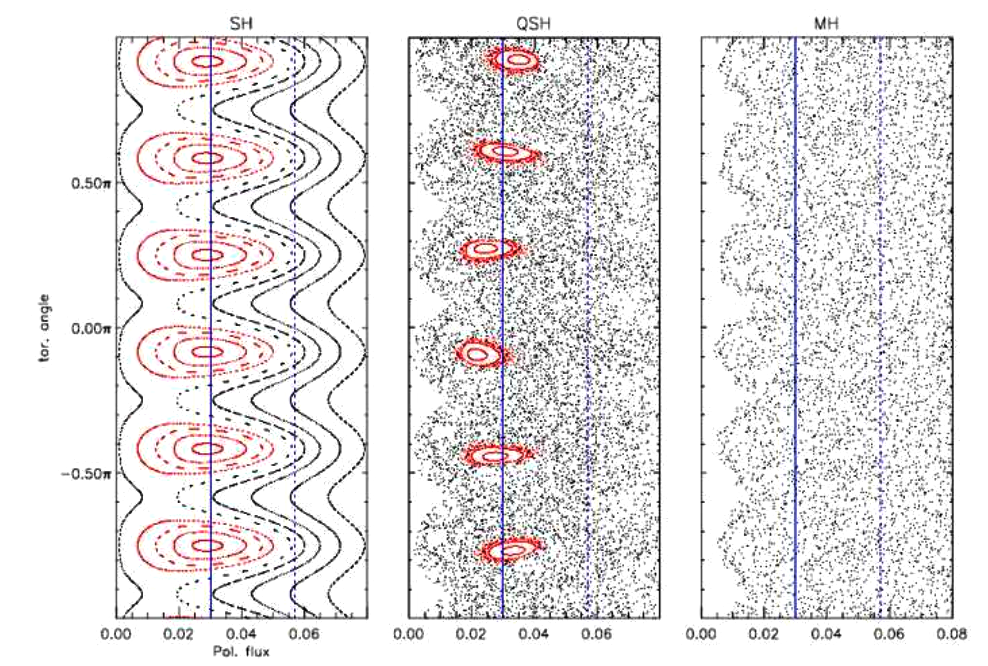
\includegraphics[height=4.2cm]{img/2_eq/poincare_QSH.png} \label{img:MHQSH_a}}
    \subfigure[]{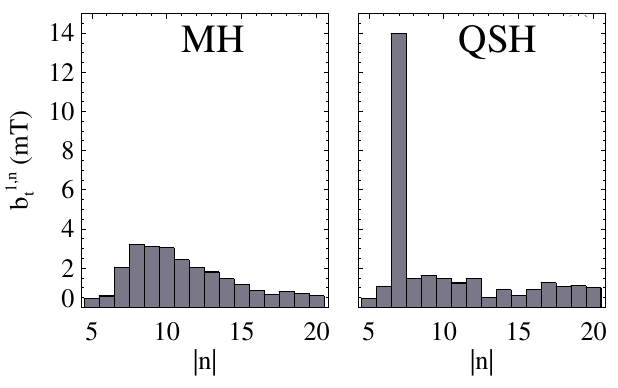
\includegraphics[height=4cm]{img/2_eq/QSH_modes_example.png} \label{img:MHQSH_b}}
    \caption{Poincaré plots of the magnetic configuration mad with ORBIT code (a) with SH, QSH, MH magnetic mode configuration     respectively; an example of toroidal mode number spectra m = 1, n modes in a VS (Virtual Shell controlled) RFX-mod discharge (b). }
    \label{img:MHQSH}
\end{figure}















%  ____  _______  __                         _ ____  
% |  _ \|  ___\ \/ /     _ __ ___   ___   __| |___ \ 
% | |_) | |_   \  /_____| '_ ` _ \ / _ \ / _` | __) |
% |  _ <|  _|  /  \_____| | | | | | (_) | (_| |/ __/ 
% |_| \_\_|   /_/\_\    |_| |_| |_|\___/ \__,_|_____|

\section{RFX-mod2 \\ \small{a chance for a better controllable machine}}
\cite{SONATO2003161}
\cite{doi:10.1063/1.4806765}
\cite{martin_RFX_overview}

% CHALLENGES AND SOLUTIONS IN THE DESIGN OF RFX-MOD2, A MULTI CONFIGURATION MAGNETIC CONFINEMENT EXPERIMENTAL DEVICE

% RWR
RFX-mod is a flexible \ac{RFP} toroidal device (major radius $R=2 m$ and minor radius $a=0.46 m$) with plasma current up to 2 MA and volume $10 m^3$ \cite{SONATO200597}. As in all RFPs, plasma heating is purely ohmic; \acl{RFP} could in principle obtain fusion power with ohmic heating only, and with a magnetic field much smaller than in a tokamak—avoiding superconducting coils. RFX-mod is equipped with a very powerful system of active coils for feedback control of plasma MHD stability: 192 coils, independently driven, cover the whole plasma surface.


\section{RFX diagnostics}
% kind of RFX diagnostics
In fusion machines the number of signals to be acquired is very high, they can be classified by the nature of the diagnostics:
signals from magnetic probes, from Soft X-Ray detectors, from light sensors such as photodiodes amd photomultipliers, from Langmuir probes, etc.
%
We can further divide the diagnostics into 4 main families:
\begin{itemize}
    \item Magnetics, and the related plasma current, loop potentials, etc.
    \item Spectroscopic diagnostics, which measure the spontaneous e.m. radiaton emitted by the plasma, ranging from the microwaves (electron cyclotron emission, ECE) to X-Ray, with all sorts in between: infrared, visible, UV and XUV. 
    \item Reflectometers and interferometers, which are based on the modification on the phase and polarization of an microwave coherent beam or optical laser, once they pass through the plasma.  
    \item Measurement of electron temperature Te provided by the light diffused by Thomson scattering (TS) when an intense laser pulse illuminates the plasma.
\end{itemize}

%
\begin{figure}[ht!]
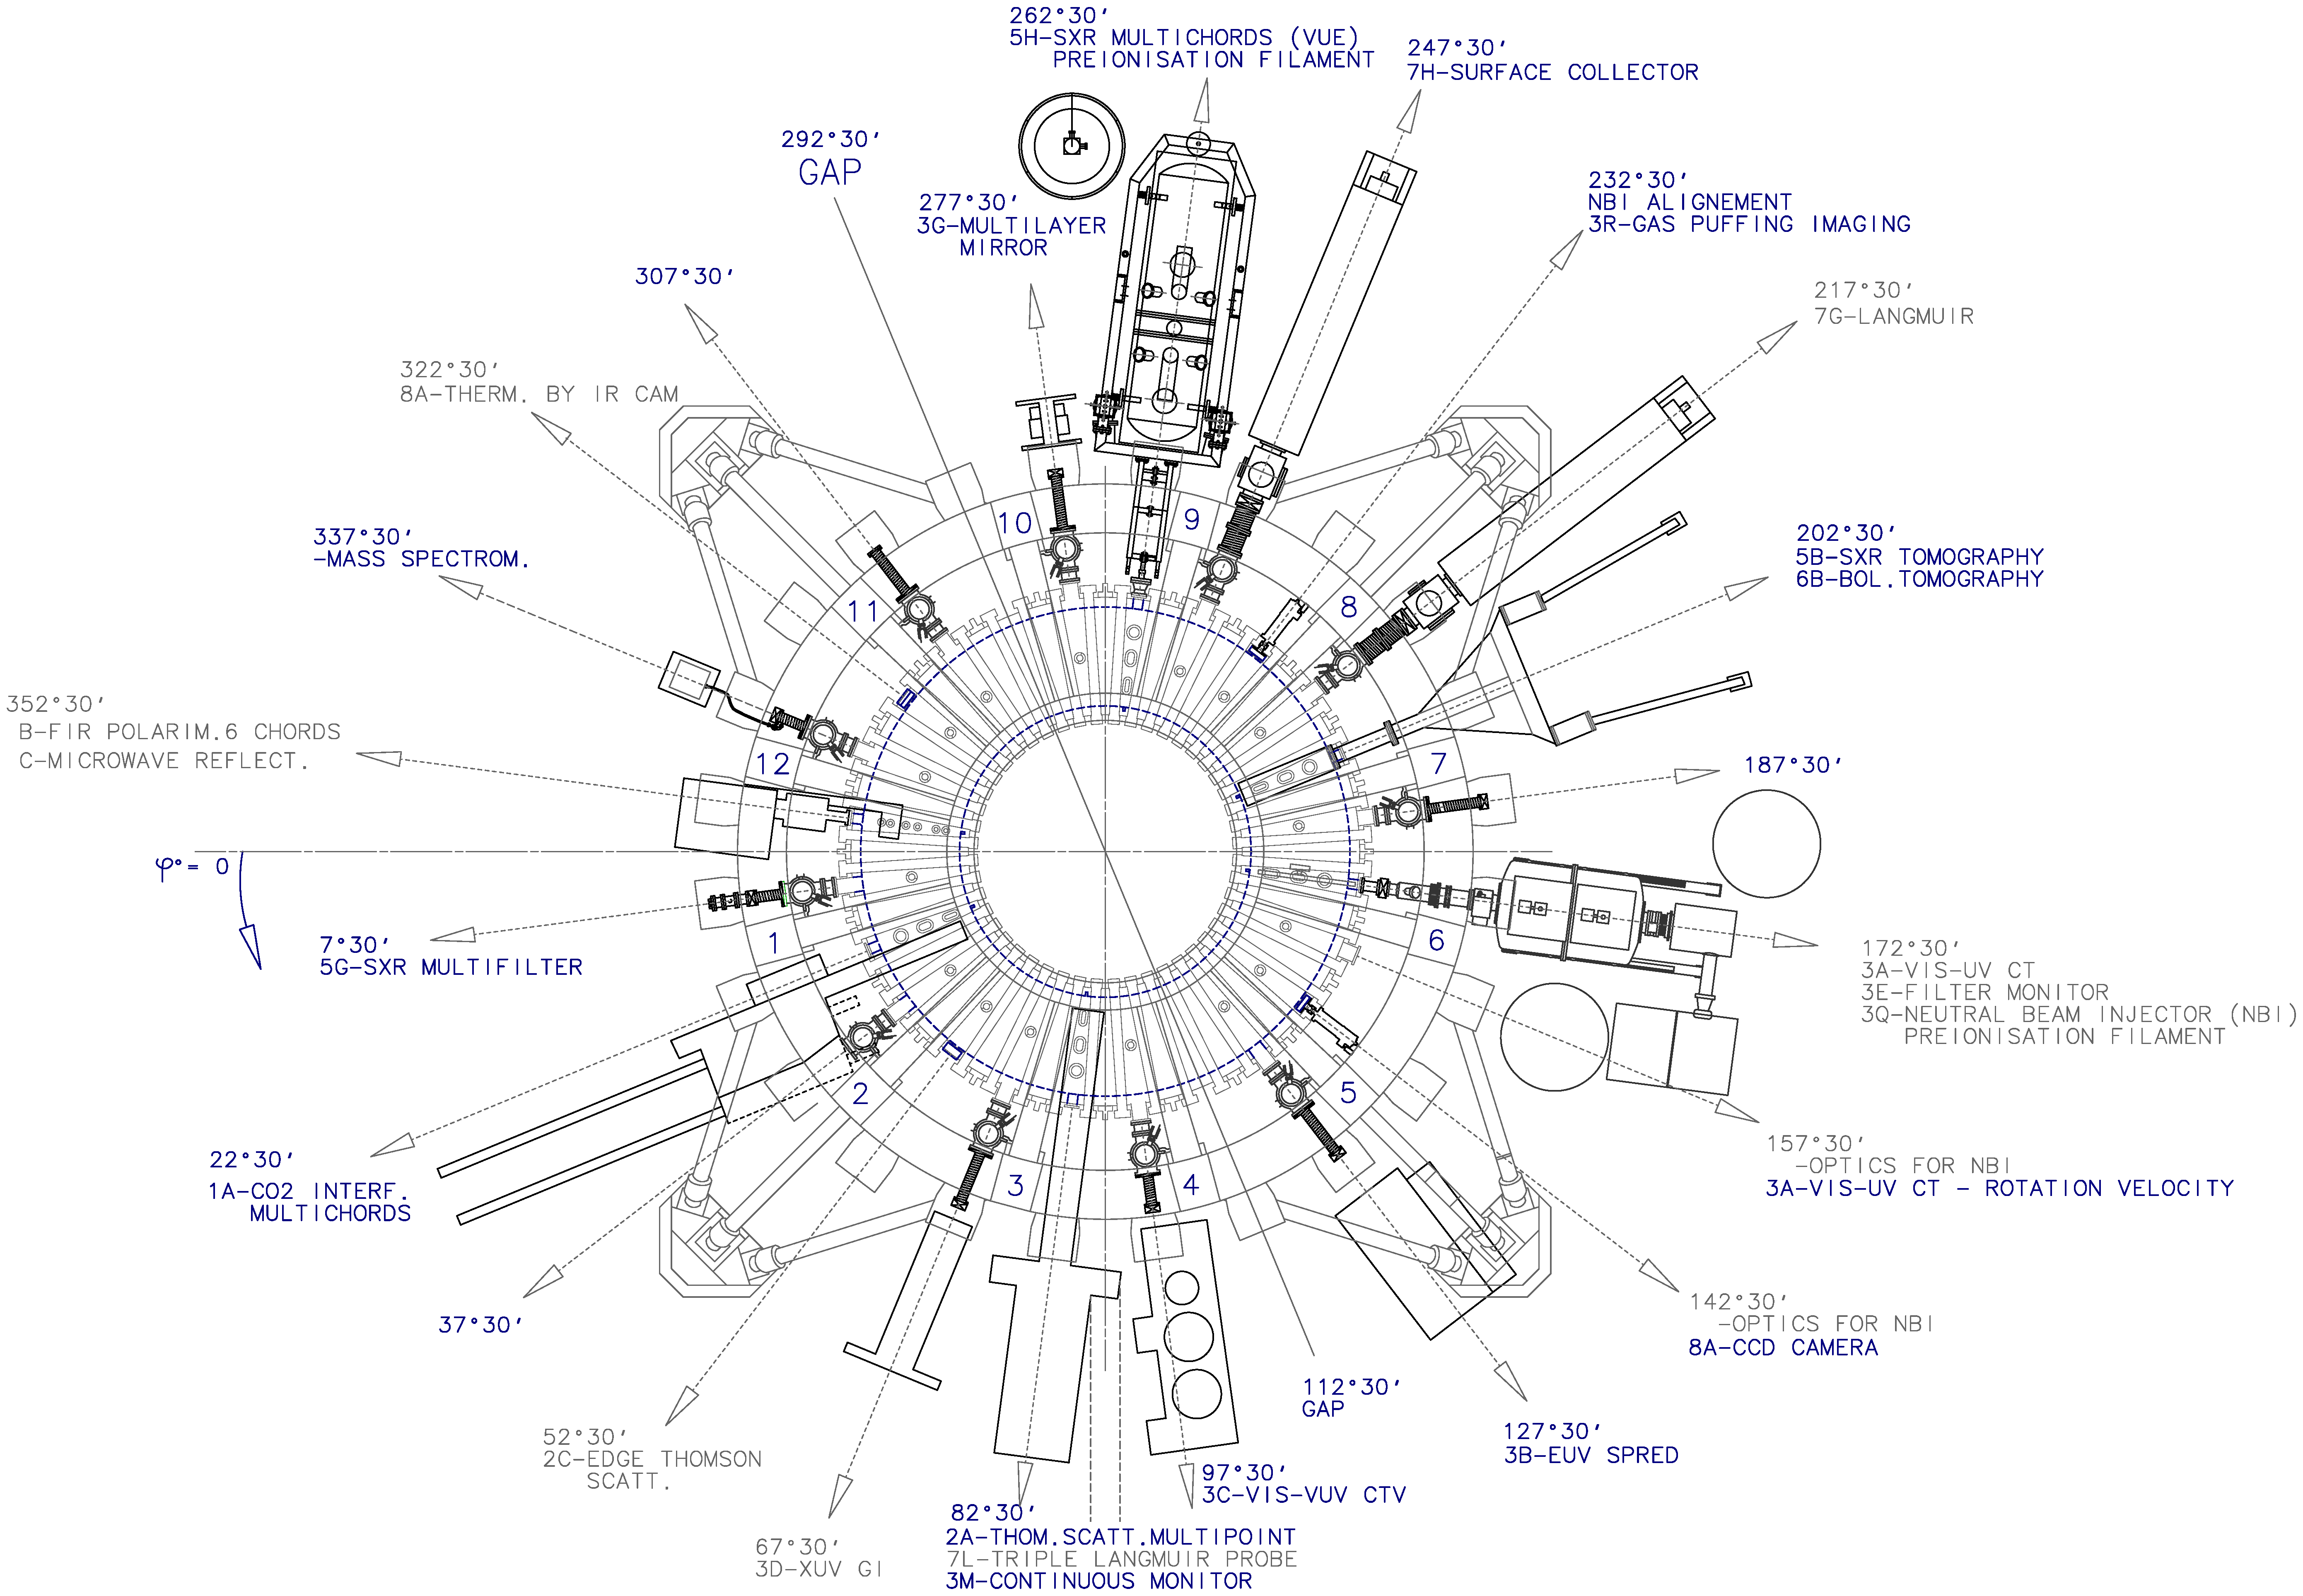
\includegraphics[width=1\textwidth]{img/rfx/Layout_Diagnosiche_AA10005.eps} \centering
% TODO: add figures
\caption{RFX map of diagnostics with related toroidal position.}
\label{rfx}
\end{figure}
%

\subsection{Thomson Scattering}
The Thomson scattering  has been a key-factor diagnostic at RFX since the initial operations for the study of RFP plasma configuration, yielding a fundamental correlation between the electron temperature and the magnetic fluctuations that link the plasma confinement to the dynamo related modes. This also evolved in the possibility to identify a hot asymmetric island when the temperature gradient extends to the plasma core in the \ac{QSH} state.
During the first operation of RFX the diagnostic was composed by a single pulse of laser from ruby diode ( $\lambda = 694 nm$ ) passing through the plasma in the equatorial plane, and two grating photo-multipliers spectrometers.
This apparatus presented some limitations: from the precision point of view it suffered of a poor quantum efficiency of the multialkali cathode of the photo-multiplier (MCP-PMT) resulting in a general lack of sensitivity and noisy profile at low electron temperatures. On the other hand the 20 chords acquisition that characterized the acquired profile with a 24 mm spatial resolution was unable to effectively investigate the details of the QSH magnetic islands.

Since the 2005 with the experiment upgrade to RFX-mod the diagnostic was completely renewed. In particular the replacement of the grating spectrometers with a set of four filter polycromators with avalanche photo-diodes (APD) provided a 30 times higher sensitivity and 84 points profile with a new narrow grained 7mm resolution ( $r/a$ from -0.96 to 0.84 ).
The new Nd:YLF laser diode ($\lambda=1053 nm$) located 15 m away from the center of the vacuum vessel, can produce an up to 7 J burst of 10 pulses per experiment shot. with a single light emission duration of 20ns FWHM (full-width at half maximum).

The light passing through plasma on the equatorial plane scatter in all directions and is collected by photo-multipliers at three different windows at the end of short vertical ports. The 84 pairs of quartz fibers look at all the plasma poloidal angles by magnifying optics located at the ports. All fibers can be also moved by a special mechanical support that can self orient during the experiment setup state; at the same time all optics can also automatically adjust focus to the desired radial position of interest.
A further side by side light path decomposes the acquired spectrum in 4 channels using a series of relay lenses.
%
The small amount of the solid angle covered by the acquisition, together with all this set of filters applied both at the input beam - aiming at reducing the stray light and maintaining the focus -, and at the output - for the selection of the plasma region of interest and for the decomposition of the energy spectrum - are the main reason for the required high power input.
%
This leads to a scattered set of acquisition pulses that are not continuously reconstructing the overall shape of plasma temperature but they are reduced to a small set of usually 10 time events per pulse.
%
The recording system is also quite complex: for RFX-mod the detected signal has been acquired by a modular 4-channels cPCI board dedicated for each of the spectrometers, acquiring data at 500 Msps each.

\subsection{Soft X Ray}

% We chose the most reliable and fast response diagnostics ... (SXR and Magnetic coils MHD)
% Other possible diagnostics can be added ( cope with time dim )
% Possibility to trigger in realtime other diagnostics ( i.e. Thomson Scattering )
The measurement of the Thomoson scattering are very precise, but are available only at few times during the shots and thus is not possible to follow the time evolution of the temperature.
A continuous measurement of the temperature can be obtained from a soft X-ray (SXR) detection system. In 1996 a SXR tomographic system was installed in a RFP (Reversed Field
Pinch) experiment for the first time \cite{Franz_2001}. 
As shown in the previous sections the RFP configuration is keen to produce a large amount of magnetic instabilities due to the low profile of the safety factor. The current driven instabilities that are very common in RFPs can grow in the core of plasma producing the so called ``magnetic islands''. 
At the islands toroidal positions the SXR emits more, and localized regions are identified. 
Imaging of these SXR structures was allowed by the application of the Fourier-Bessel expansion of the Cormack inversion, as proposed by Nagayama in~\cite{Bonomo25}. 
The algorithm is studied to achieve a good image reconstruction even with few harmonics, as the case of SXR where the acceptance of integral measuring cords  is affected by the small (and few) openings in the vessel. If the amplitude of the many magnetic instabilities is approximately the same, as in the case of the so-called \acl{MH}, the reconstructed SXR emissivity is almost symmetric; it is shown in~\Figure{\ref{fig:MH_QSH_example}a}. Conversely, in presence of an instability where a single mode dominates, a magnetic island is sustained and, as shown in~\Figure{\ref{fig:MH_QSH_example}b}, an asymmetric emissivity profile with a localized bight region is detected. This state is called \acl{QSH}.
%
\begin{figure}
    \centering
    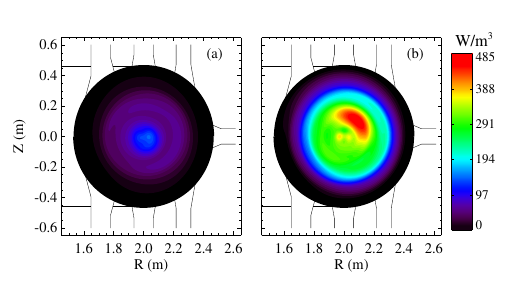
\includegraphics[height=5cm]{img/2_eq/MH_QSH_example.png}
    \caption{Contour plot of the reconstructed SXR emissivity for a standard multiple helicity (MH) configuration (a), and for a quasi-single helicity (QSH) configuration (b); acquired at RFX by SXR3 device; the color bar is in W /m3 .
    }
    \label{fig:MH_QSH_example}
\end{figure}
%
In the currently operating RFP experiments, and in RFX-mod likewise, the time evolution of such instabilities is of the order of few ms. This sets a requirement on the bandwidth of the measurements up to several hundreds of kHz.

A new SXR diagnostic named DSX3 have been installed in one of the equatorial ports of RFX-mod chamber; it completes the existing tomographic diagnostic maintaining several primary characteristics of the original SXR manipulators. Further
features have been added: a larger number of acquired cords, a wider flexibility in the detection system geometry and the possibility of dynamically selecting different ranges of detected radiation energy.
%
\begin{figure}
    \centering
    \subfigure[]{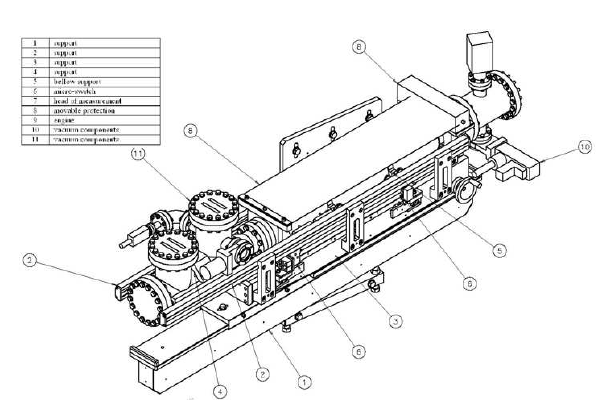
\includegraphics[height=5cm]{img/rfx/SXR_sketch.png}}
    \subfigure[]{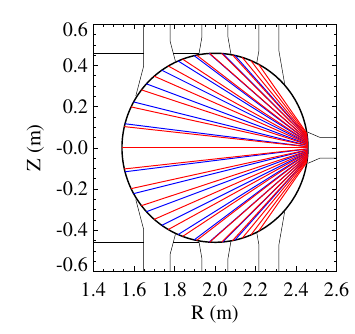
\includegraphics[height=5cm]{img/rfx/SXR3_cords.png}}
    \caption{DXS3 perspective view (a), and the geometry of the lines of sight of DSX3 (at the tomography toroidal section
             of RFX-mod vessel) for the three rows of photodiodes (b): the red lines correspond to the
             27 diodes of the central row, while the chords for the two external rows (blue lines) are perfectly
             overlapping }
    \label{fig:DSX3_sketch}
\end{figure}




% \section{The complete “SCHEMA” from sensors to plasma parameters}

% \chapter{RFP Equilibrium}
% \section{MHD}
% \section{Newcomb SH}
% \section{The complete “SCHEMA” from sensors to plasma parameters}

\chapter{Machine Learning and Latent Space Equilibrium}

As previously described in the introductory chapter of this manuscript we have been spectators of a deep advance in the computation technology in this decade that opened for data-science the era of \textbf{big data}. For example there are millions of autonomous software components that continuously crawl the internet network decoding HTML pages from 60 billion of pages collected and indexed in a single database. Each time we capture a picture this file is automatically classified and stored in a cloud space that is claimed to receive 1.2 billion of pictures per day. 

We can define ML as the available set of tools that analyzing such big amount of information are automatically providing a possible uncovered pattern among them to be eventually able to predict a future output of the system and operate any other kind of decision based on data uncertainty. The intimate meaning of \textit{machine learning} in this context is referred to the fact that the human intervention is on the very base of the algorithm structural definition while it is the actual model itself that stitches to the input data.  
%
In science, there are essentially two modelling approaches: \textbf{data driven models}; and \textbf{process based models}.
Although physical modeling is the main primary tool to understand the behaviour of natural processes, and to make inference about the future outcomes, it is becoming an increasingly exploited solution to employ a data driven approach where the process based physical models appear to be not detailed enough to describe complex systems in operational situations. For instance we often look at the sole main physical phenomenon where the output measured quantities are actually corrupted by non linear cascade of underlying effects, or we are even looking at an unknown behavior for witch the model results to be a partial or wrong description for the actual measured representation. 
In some other cases, a hybrid version of combined physical and statistical model could be also explored, as we will see in the next sections. But the actual point is that we start to look at the measures of an experiment, not only from the perspective of the single independent experience but from a more general point of view that takes into account the whole repetition history and a wider operational space.  



\section{Statistical description of DNN}

As already anticipated, in order to gather a wide range of all the possible concurring physical causes that drive the measures, we decided to make use of the latest novel approach of Deep Neural Networks. As a preliminary backward step, this section would provide a slight general description that bases this approach in a statistical oriented fashion. Indeed this is the preferred mathematical representation of the recurrent/repeatable output of a scientific experiment lead by the probability theory as it was generalized by Pierre Laplace (1812). 

The collated set of all measures along the consecutive experimental repetitions is often referred as the model \textit{dataset}, while a single instance of this dataset with a proper selection of the quantities under analysis is commonly called \textit{features} or \textit{covariates}\footnote{The most precise definition seems to be the term covariate used in Analysis of Covariance, a type of General Linear Model in which the independent variables of interest are categorical, but you also need to adjust for the effect of an observed, continuous variable–the covariate}.
%
If we consider our dataset in the generic physical model outputs we can refer as the single input feature of the ML model as a stochastic vector $\bm{x} = [x_1,x_2, ... ,x_N]$ that is characterized by its probability density distribution $p(\bm{x})$. The very general macroscopic description of any machine learning application consists to feed a statistical model with this input feature eventually providing as output the \textit{p.d.f} of another related measure $p(y|\bm{x})$ or a description of $p(\bm{x})$ itself. These two kinds of results are respectively representative of the so called  \textbf{supervised} and \textbf{unsupervised} learning: in the former the the model is confronted with a known relation between variables, while any information is provided to the model for the latter but we are simply looking at the distribution of the variables in their own manifold or in a subspace (as it will described in the next sections).

The unitary element that composes either the standard \textit{Neural Network} structure and the \textit{Deep Neural Network} is the so called \textit{Single Layer Perceptron}; in the following it will be shown that this particular element can be seen as a single instance of a \ac{GLM}, while the operation performed by each of this quantity is a generic regression model applied on its input features.
%
Although GLM is the generalized representation of the ordinary linear regression we shall first introduce the latter as a first example to present the formalism in a simpler manner.
The very basic linear regression model is a linear mapping from N-dimensional input features (or covariates) $\bm{x}$, to a set of targets (or responses) $\bm{y}$, using the inputs, a set of weights (or regression coefficients) $\bm{w}$ and a bias offset $w_0$. The internal product of features and weights gives the equation of the fitter that in the linear form has the shape of a line in the N-dimensional space. The line is centered within the input data while typically the probabilistic model assumes that the residuals can be described with a Gaussian shape of unknown variance $\sigma^2$. The model can be written as a predictor in the form:
\begin{equation}
    \hat{y} = \eta + \epsilon
\end{equation}
where
\begin{equation}
     \eta = \transpose{\bm{w}}\bm{x} \qquad  \epsilon \in \mathcal{N}(0,\sigma^2)
\end{equation}
the first addendum is the \textit{linear predictor} in which a scalar is appended at the end of the the weight vector to fit the bias of the distribution, and the second addendum represents the overall error. To let the model fitting also the bias the parameters and covariates array have been rewritten as follows:
\begin{equation}
    \bm{w} = [\hat{\bm{w}},w_0] \qquad \bm{x} = [\hat{x}, 1]
\end{equation}
At this point the conditional probability of the target given the features can be modeled as a Gaussian distribution:
\begin{equation}
    p(y|\bm{x}) = \mathcal{N}(\eta, \sigma^2)
\end{equation}
this happens because we forced to consider the features with normal distribution and because being an exponential distribution it is also a conjugate prior for the likelihood, as it will described in the following.

\subsection{Generalized Linear Models}
The use of exponential distribution turns to be a very clever solution. Indeed, among all families of distributions, where the definition domain does not vary with the parameter being estimated, this family is the only one with a sufficient statistic whose dimension remains bounded if the sample size increases. This means that we can have a compressed representation of the dataset into a fixed size summary without loss of information.
Exponential families are also important in Bayesian reconstruction where a prior distribution is multiplied by a likelihood function and normalised to produce the posterior. In the case of a likelihood which belongs to an exponential family there always exists a conjugate prior, which is usually also exponentially distributed. 
%
%A conjugate prior for the parameter $\eta$ of an exponential family
The formal definition of a generic exponentially distributed p.d.f. is the following:
%% EXPONENTIAL
\begin{equation}
    p(x|\theta) = \frac{1}{Z(\bm{\theta})}h(x) \exp{[\transpose{\bm{\theta}} \phi(\bm{x})]}
\end{equation}
where $\bm{\theta} \in \Theta \subseteq \mathbb{R}^d$ are defined as the \textbf{natural parameters}, $\phi(\bm{x}) \in \mathbb{R}^d$ is called the vector of \textbf{sufficient statistics}, $h(\bm{x})$ is a scaling factor that is usually a unitary constant, and $Z(\bm{\theta})$ is the \textbf{partition function} that normalizes the distribution:
\begin{equation}
    Z(\bm{\theta}) = 
    \int_{\mathcal{X}^n} h(\bm{x}) \exp{[\transpose{\bm{\theta}} \phi(\bm{x})]} dx
\end{equation}
Being all the arguments within an exponential operator it is also quite common to embed the partition function too, using $ A(\bm{\theta}) = \log\left(Z(\bm{\theta})\right)$ in the following:
\begin{equation}
    p(x|\bm{\theta}) = h(\bm{x}) \exp{[\transpose{\bm{\eta}}\phi(\bm{x}) - A(\bm{\eta}) ]}
\end{equation}
where the function $\eta$ has been further introduced to expand the natural parameters to the representation $\bm{\eta}=\eta(\bm{\theta})$, where $\text{dim}(\bm{\theta}) \leq \text{dim}\left(\eta(\bm{\theta})\right)$.

%% BERNOULLI EXPONENTIAL
\subsubsection*{example: exponential representation of the Bernoulli distribution}
The Bernoulli distribution for $x\in\{0,1\}$ can be written in exponential family form as:
\begin{equation}
\begin{split}
    \text{Ber}(x|\mu) &= \mu^x(1-\mu)^{1-x} \\
%                      &= (1-\mu) \exp{\left[ x \log\left(\frac{\mu}{1-\mu}\right)\right]} \\
                      &= \exp{\left[\transpose{\phi(x)}\bm{\theta} \right]}
\end{split}
\end{equation}
where we set:
\begin{align*}
  & \phi(x) = x \\
  & \theta  = \log\left(\frac{\mu}{1-\mu}\right) \\
  & Z = 1/(1-\mu)
\end{align*}

%% GAUSSIAN EXPONENTIAL
\subsubsection*{example: exponential representation of the Univariate Gaussian distribution}
The univariate Gaussian can be written in exponential family in this form:
\begin{equation}
\begin{split}
        \mathcal{N}(x|\mu,\sigma^2) &= \frac{1}{(2\pi\sigma^2)^\frac{1}{2}} \exp{\left[-\frac{1}{2\sigma^2}(x-\mu)^2\right]} \\
        & \frac{1}{Z(\bm{\theta}}\exp{\left[\transpose{\bm{\theta}}\bm{\phi}(x)\right]}
\end{split}
\end{equation}
once the parameters have been set to:
\begin{align*}
    & \bm{\phi}(x) = \left[ x, x^2 \right] \\
    & \bm{\theta}  = \left[ \frac{\mu}{\sigma^2}, -\frac{1}{2\sigma^2} \right] \\
    & Z(\mu,\sigma^2) = \sqrt{{2\pi\sigma^2}} \exp{\left[ \frac{\mu^2}{2\sigma^2} \right]}
\end{align*}

%%GLM
It has been shown that the linear regression predicts the expected value of a given quantity as a linear combination the dataset. This implies that a constant change in the covariates leads also to a constant change in the response (i.e. a linear-response model). This is appropriate when the response variable has a normal distribution (intuitively, when a response variable can vary essentially indefinitely in either direction with no fixed "zero value", or more generally for any quantity that only varies by a relatively small amount).
However, these assumptions are inappropriate where the response variable is expected to have a different shape. 
% RR
As an example, a prediction model might predict that 10 degree temperature decrease would lead to 1,000 fewer people visiting the beach is unlikely to generalize well over both small beaches (e.g. those where the expected attendance was 50 at a particular temperature) and large beaches (e.g. those where the expected attendance was 10,000 at a low temperature). The problem with this kind of prediction model would imply a temperature drop of 10 degrees would lead to 1,000 fewer people visiting the beach, a beach whose expected attendance was 50 at a higher temperature would now be predicted to have the impossible attendance value of -950. Logically, a more realistic model would instead predict a constant rate of increased beach attendance (e.g. an increase in 10 degrees leads to a doubling in beach attendance, and a drop in 10 degrees leads to a halving in attendance). Such a model is termed an exponential-response model (or log-linear model, since the logarithm of the response is predicted to vary linearly).
%% 
Generalized linear models overcome this limitation extending the ordinary linear models expanding the response variables to any arbitrary distribution (rather than simply the normal), imposing an arbitrary function of the response variable (the link function) to exploit the linearity with the predicted values. 
% RR
For example, the case above of predicted number of beach attendees would typically be modeled with a Poisson distribution and a log link, while the case of predicted probability of beach attendance would typically be modeled with a Bernoulli distribution (or binomial distribution, depending on exactly how the problem is phrased) and a log-odds (or logit) link function.
%%GLM
The three main ingredients of a GLM are:
\begin{itemize}
    \item The \textbf{exponential family} of probability distributions,
    \item the usual \textbf{linear predictor} $\eta = \transpose{\bm{w}}\bm{x}$,
    \item a \textbf{link function} $g$ such that $\expectation{y|\bm{x}} = \mu = g^{-1}(\eta)$.
\end{itemize}

The GLM probability is composed as follows:
\begin{equation}
    p(y_i| \theta, \sigma^2) = 
    \exp{\left[ \frac{y_i\theta - A(\theta}{\sigma^2} + c(y_i,\sigma^2) \right] }
\end{equation}


%
%  _____ ___ _     _       _   _ _____ ____  _____ 
% |  ___|_ _| |   | |     | | | | ____|  _ \| ____|
% | |_   | || |   | |     | |_| |  _| | |_) |  _|  
% |  _|  | || |___| |___  |  _  | |___|  _ <| |___ 
% |_|   |___|_____|_____| |_| |_|_____|_| \_\_____|
%

%% GLM

%% GAUSSIAN MODEL EXAMPLE

%% CLOSED FORM FOR GAUSSIAN MODEL

\subsection{Directed Graphical Models}
In the previous chapter we saw a possible general approach to obtain a regression of a single target variable given its conditional probability with an input process. Suppose now that we are observing a set of multiple correlated variables where the correlation extends from one variable to another in a chain of dependencies. This becomes a stochastic model describing a sequence of possible values for the variables in which the probability of each event depends on the state of the others.
If we constrain the variable correlation to be strictly ordered the probability of a target variable after all the correlation hops can be written as:
\begin{equation}
    p(x_1, x_2, ... x_V | \bm{\theta}) = p(x_1|\bm{\theta})p(x_2|x_1,\bm{\theta})p(x_3|x_2,x_1,\bm{\theta}) ... p(x_V|x_1, ... x_{V-1},\bm{\theta})
\end{equation}
Looking at all the possible $p(x_i|\bm{\theta})$ the conditional links among variable appears as a linked directed graph.
%
This is called “Graphical model” as it combines graph theory and probability theory to provide a general framework to represent variables interaction. Graphical models trace their origins to many different fields and have been applied in wide variety of settings: for example, to develop probabilistic expert systems, and to understand neural networks. Remarkably, the very same formalism and algorithms can be applied to a wide range of problems.
%
However even if the pictorial result is quite intuitive, the joint relation among stochastic variables can easily grow exponentially; for instance if we imagine all distributions having the same finite discrete support composed by $K$ states the representation of all $p(x_i|x_j)$ is $O(K^2)$, the representation of $p(x_i|x_j,x_k)$ is $O(K^3)$ and so forth, so the overall model of V cardinality would become $O(K^V)$. This description of joint discrete possible states, known as the \textbf{conditional probability table}, is sometimes used to describe a fully observed covariates vector in the complete statistical description of the complex systems of variable. Actually this solution, beside requiring a first restriction in the number of possible states that represents each stochastic process, it is also presenting a critical convergence requiring a awful amount of data to reach a meaningful state for such amount of parameters.
One possible solution, in the same discrete approximation, is to make use a more compact conditional distribution function, such as the multinomial logistic i.e. $p(x_i | \bm{x_j})_{i \neq j} = S_k(\bm{W}_i \bm{x_{j}}$). Although this model has been successfully applied in literature for some generative classifiers~\cite{Bengio:1999:MHD:3009657.3009714}, it appears to remain an overkill in conditioning the system.

Another practical end very common solution is to assume a conditional Independence among variables that are k-hops distant from the others, exploiting the \textbf{Markov assumption} of independence among the link graph.
For example, under these conditions, imposing a single hop Independence, the chains of links that create are constituted by first order \textbf{Markov chain} shown in the first diagram of \Figure{\ref{fig:simple_markov_chains_a}}, and described by the following joint distribution:
\begin{equation}
    p(x_1, x_2, ... x_V) = p(x_1) \prod_{j=1}^V p(x_j|x_{j-1})
\end{equation}
equivalently the second order independence can be imposed, generating a graph like in \Figure{\ref{fig:simple_markov_chains_b}} describe by:
\begin{equation}
    p(x_1, x_2, ... x_V) = p(x_1) \prod_{j=1}^V p(x_j|x_{j-1},x_{j-2})
\end{equation}
In the same way higher-order Markov models can be created, however even the second-order Markov assumption may be inadequate if there are long-range correlations throughout the available observations since the number of parameters will again blow up. 





\begin{figure}
    \centering
    \subfigure[]{
    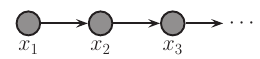
\includegraphics[width=0.3\textwidth]{img/3_ML/DGM_o1_markov.png}
    \label{fig:simple_markov_chains_a} }
    \subfigure[]{
    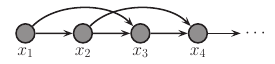
\includegraphics[width=0.3\textwidth]{img/3_ML/DGM_o2_markov.png}
    \label{fig:simple_markov_chains_b} }
    \caption{First order (a) and second order (b) Markov Chain examples, the arrow represents a conditional probability that relates variables each other.}
    \label{fig:simple_markov_chains}
\end{figure}

\begin{figure}
    \centering
    \subfigure[]{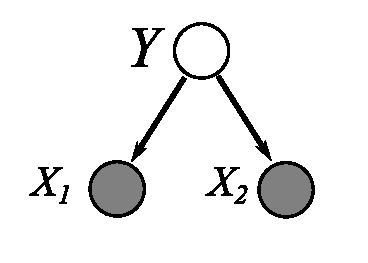
\includegraphics[height=2cm]{img/3_ML/naive_bayes_1.pdf}
    \label{fignaive_bayes}}
    \subfigure[]{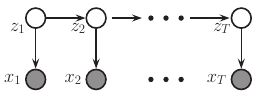
\includegraphics[height=2cm]{img/3_ML/DGM_o1_hmm.png}
    \label{fig:hidden_markov}}
    \caption{Caption}
\end{figure}

A further possible reduction in the number of joint relations between observed variables can be also given by the formalism itself,  by the assumption that some covariates are correlated because they all arise from a hidden common “cause”. Those common causes are variables themselves that can't be directly measured.  Model with hidden variables are also known as latent variable models or LVMs. 

The actual very powerful alternative approach is to assume that there is an underlying hidden process, that can be modeled by a first-order Markov chain, but for which available measures is a noisy observation of this process. The result is known as \acl{HMM}, shown in \Figure{\ref{fig:hidden_markov}}. 










%  _____ _____ ____  _   _      _                      _    
% |  ___|  ___|  _ \| \ | | ___| |___      _____  _ __| | __
% | |_  | |_  | | | |  \| |/ _ \ __\ \ /\ / / _ \| '__| |/ /
% |  _| |  _| | |_| | |\  |  __/ |_ \ V  V / (_) | |  |   < 
% |_|   |_|   |____/|_| \_|\___|\__| \_/\_/ \___/|_|  |_|\_\

\subsection{Feed forward dense network}
%
A feed forward NN, aka \ac{MLP} is again using the linear regression, actually it can be seen as a chain of logistic regression models that are stacked one on top of each other, where the final layer being either a logistic or a linear regression depending weather we are looking for a general classification output (i.e. a probability function output for each of the classes in the classifier domain) or a regression output. 
For instance, looking at the simple two layers example, and considering a regression output problem, the model would be written like:
\begin{equation}
    p(y|\bm{x},\bm{\theta}) = \mathcal{N}\left(y|\transpose{\bm{w}}\bm{z(\bm{x}}), \sigma^2 \right)
\end{equation}
where the basis function expansion here is a non-linear response of further linear combination of the inputs:
\begin{equation}
    \bm{z}(\bm{x}) = \left[ g(\transpose{\bm{v}_1}\bm{x}), g(\transpose{\bm{v}_2}\bm{x}), ..., g(\transpose{\bm{v}_H}\bm{x}) \right]
\end{equation}
the transformation $z(\bm{x})$ represents here the non-linear transformation on regression in which the deterministic function $g(\bm{x},\bm{v})$, also called the \textbf{activation function}, is the kernel of the basis function expansion. In this way we could think of the MLP as a kernel machine where the kernel functions are opportunely shaped to match the input data, this is indeed referred as an \textbf{adaptive basis function model} where the entire parameter set that embrace the kernel parameters is: $\bm{\theta} = (\bm{w}, \bm{v})$ with $\bm{w} = [w_0, w_1, ..., w_D]$ and $\bm{v} = [v_1, v_2, ..., v_H]$

\begin{figure}
    \centering
    \subfigure[]{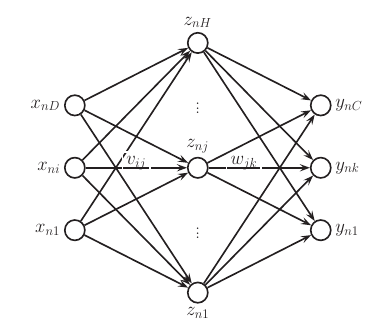
\includegraphics[height=4cm]{img/3_ML/MLP.png} \label{fig:mlp_a}}
    \subfigure[]{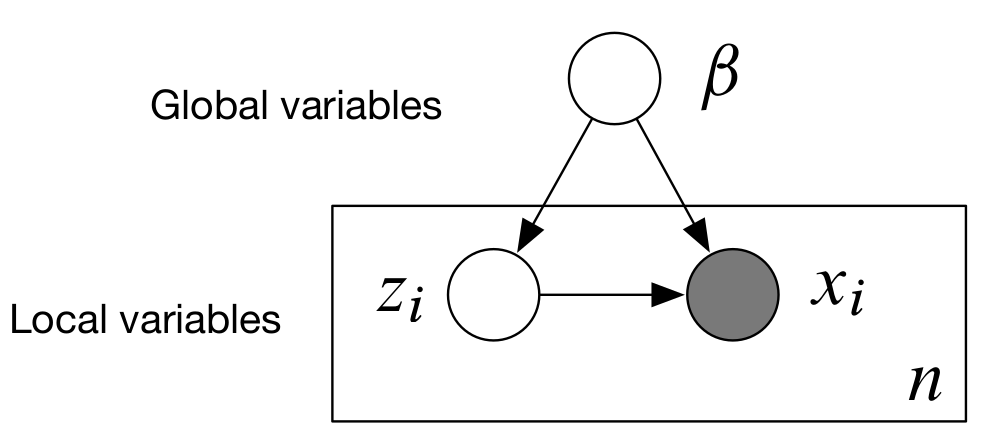
\includegraphics[height=4cm]{img/3_ML/FDN_plate_model.png}}
    \caption{One hidden layer Feed Forward Neural Network (or equivalently the minimal Multi Layer Perceptron, seen as an Adaptive Basis Function Model (a), and the equivalent model in plate notation (b). }
    \label{fig:mlp}
\end{figure}

The overall GLM applied can be constructed as usual in many different shapes, depending on the target type of inference we are interested in. If we look for a binary classification it appears as a logistic regression, i.e. the fit on the Bernoulli distribution of the sigmoid outputs:
\begin{equation}
    p(y|\bm{x}, \bm{\theta}) = \text{Ber}\left( y|\text{sigm}(\transpose{\bm{w}}\bm{z}(\bm{x}) \right)
\end{equation}
If we are looking for categorical classifier the correct GLM has to be distributed as:
\begin{equation}
    p(y|\bm{x}, \bm{\theta}) = \text{Cat}\left( y|\mathcal{S}(\transpose{\bm{w}}\bm{z}(\bm{x})) \right)
\end{equation}
where the \textit{Cat} distribution is the Multinulli and $\mathcal{S}$ stands for the support function of the input.
Finally as stated in the first example if we are fitting a generic output function it will appear for example as a Gaussian regression model:
\begin{equation}
    p(\bm{y}|\bm{x}, \bm{\theta}) = \mathcal{N}\left( \bm{y}|\bm{W} \phi \right)
\end{equation}
where in this last version of the formula the probability has been shaped with the weights matrix $\bm{W}$ taking into account the possible MIMO configuration of the perceprton as shown in \Figure{\ref{fig:mlp_a}}.
It is finally a key factor for the activation function $g(\bm{x},\bm{v})$ to be a non-linear operator because the overall network would collapse into a large linear regression otherwise. Usually the activation is the logistic function $g(u) = \text{sigm}(u)$ or the recently much common flavors of the \textbf{rectified linear units} (ReLU) that provide a non linear activation with a minimal computational effort.
% 
All this kind of complication that have been added to the simple GLM are actually building a problem of optimization, to find the best functional fit for a set of input-output examples. So we are tuning the weights to chase for an optimal configuration; but two complementary motivations determine what \textit{optimal} means in this context. On the one hand we want the network to represent the target as exactly as possible. But on the other hand the network must be capable of generalize, that is, unknown inputs must be compared to the known ones and the output produced is a kind of interpolation of learned values. However, good generalization and minimal reproduction error of the learned input-output pairs can become contradictory objectives.

\subsection{Convolutional Neural Networks}

The previous section explained how a ABFM

The purpose of the hidden units is to learn non-linear combinations of the original inputs; this
is called feature extraction or feature construction. These hidden features are then passed as
input to the final GLM. This approach is particularly useful for problems where the original input
features are not very individually informative. For example, each pixel in an image is not very
informative; it is the combination of pixels that tells us what objects are present. Conversely, for
a task such as document classification using a bag of words representation, each feature (word
count) is informative on its own, so extracting “higher order” features is less important. Not
suprisingly, then, much of the work in neural networks has been motivated by visual pattern




\section{Unsupervised learning: Generative modeling}
% RR
“Generative modeling” is a broad area of machine learning which deals with models of distributions $p(\bm{x})$, defined over datapoints X in some potentially high-dimensional space X. For instance, images are a popular kind of data for which we might create generative models. Each “datapoint” (image) has thousands or millions of dimensions (pixels), and the generative model’s job is to somehow capture the dependencies between pixels, e.g., that nearby
pixels have similar color, and are organized into objects. Exactly what it means to “capture” these dependencies depends on exactly what we want to do with the model. One straightforward kind of generative model simply allows us to compute P(X) numerically. In the case of images, X values  which look like real images should get high probability, whereas images that look like random noise should get low probability. However, models like this are not necessarily useful: knowing that one image is unlikely does not help us synthesize one that is likely. Instead, one often cares about producing more examples that are like those already in a database, but not exactly the same. We could start with a database of raw images and synthesize new, unseen images. We might take in a database of 3D models of something like plants and produce more of them to fill a forest in a video game. We could take handwritten text and try to produce more handwritten text. Tools like this might actually be useful for graphic designers. We can formalize this setup by saying that we get examples X distributed according to some unknown distribution Pgt(X), and our goal is to learn a model P which we can sample from, such that P is as similar as possible to Pgt.

\subsubsection{Mixture models}



\subsubsection{linear factor analysis}

One problem with mixture models is that they only use a single latent variable to generate the
observations. In particular, each observation can only come from one of K prototypes. One can
think of a mixture model as using K hidden binary variables, representing a one-hot encoding
of the cluster identity. But because these variables are mutually exclusive, the model is still
limited in its representational power.
An alternative is to use a vector of real-valued latent variables, $z_i \in R_L$ . The simplest prior
to use is a Gaussian (we will consider other choices later):

% p(zi ) = N (zi |μ0 , Σ0 )

If the observations are also continuous, so $x_i \in R_D$ , we may use a Gaussian for the likelihood.
Just as in linear regression, we will assume the mean is a linear function of the (hidden) inputs,
thus yielding




% RR  VAE
Training this type of model has been a long-standing problem in the machine learning community, and classically, most approaches have had one of three serious drawbacks. First, they might require strong assumptions about the structure in the data. Second, they might make severe approximations, leading to sub optimal models. Or third, they might rely on computationally expensive inference procedures like Markov Chain Monte Carlo. More recently, some works have made tremendous progress in training neural networks as powerful function approximators through backpropagation \cite{NIPS2012_4824}. These advances have given rise to promising frameworks which can use backpropagation-based function approximators to build generative models. One of the most popular such frameworks is the Variational Autoencoder \cite{}, the subject of this tutorial. The assumptions of this model are weak, and training is fast via backpropagation. VAEs do make an approximation, but the error introduced by this approximation is arguably small given high-capacity models. These characteristics have contributed to a quick rise in their popularity

% RR
An autoencoder is a neural network that is trained to attempt to copy its input to its output. Internally, it has a hidden layer $h$ that describes a code used to represent the input. The network may be viewed as consisting of two parts: an encoder function $h=f(x)$ and a decoder that produces a reconstruction $r=g(h)$. If an autoencoder succeeds in simply learning to set $g(f(x))=x$ everywhere, then it is not especially useful. Instead, autoencoders are designed to be unable to learn to copy perfectly. Usually they are restricted in ways that allow them to copy only approximately, and to copy only input that resembles the training data. Because the model is forced to prioritize which aspects of the input should be copied, it often learns useful properties of the data.
%  _____ ___ _     _       _   _ _____ ____  _____ 
% |  ___|_ _| |   | |     | | | | ____|  _ \| ____|
% | |_   | || |   | |     | |_| |  _| | |_) |  _|  
% |  _|  | || |___| |___  |  _  | |___|  _ <| |___ 
% |_|   |___|_____|_____| |_| |_|_____|_| \_\_____|
%

%% ALL DIMENSIONALITY REDUCTION

% RR
Modern autoencoders have generalized the idea of an encoder and a decoder beyond deterministic functions to stochastic mappings $p_{encoder}(h | x)$ and $p_{decoder}(x | h)$.

%% TODO: TALK ABOUT GAN TOO

\subsection{Variational autoencoders and ELBO minimization}

% RR
In just three years, Variational Autoencoders (VAEs) have emerged as one of the most popular approaches to unsupervised learning of complicated distributions. VAEs are appealing because they are built on top of standard function approximators (neural networks), and can be trained with stochastic gradient descent.

% RR
Copying the input to the output may sound useless, but we are typically not interested in the output of the decoder. Instead, we hope that training the autoencoder to perform the input copying task will result in h taking on useful properties. One way to obtain useful features from the autoencoder is to constrain h to have a smaller dimension than x. An autoencoder whose code dimension is less than the input dimension is called \textbf{undercomplete}. Learning an undercomplete representation forces the autoencoder to capture the most salient features of the training data.







%  _____ ___ _     _       _   _ _____ ____  _____ 
% |  ___|_ _| |   | |     | | | | ____|  _ \| ____|
% | |_   | || |   | |     | |_| |  _| | |_) |  _|  
% |  _|  | || |___| |___  |  _  | |___|  _ <| |___ 
% |_|   |___|_____|_____| |_| |_|_____|_| \_\_____|
%


\section{Latent space topology in a simulated world}

\subsection{STEP1}

\begin{figure}
    \centering
    \subfigure{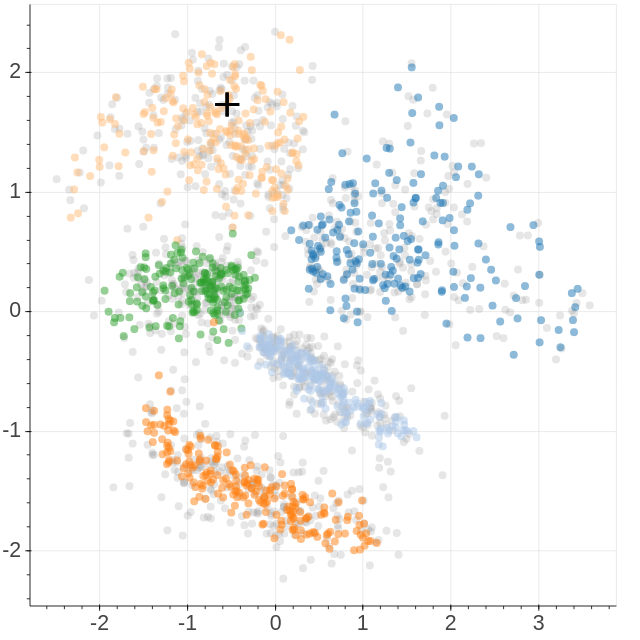
\includegraphics[height=4.5cm]{img/STEP1/ls1.png} \label{step1_1}}
    \subfigure{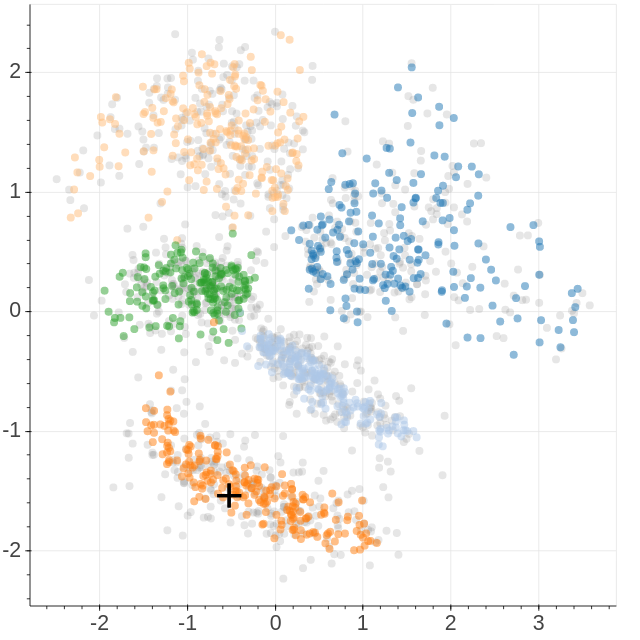
\includegraphics[height=4.5cm]{img/STEP1/ls2.png} \label{step1_2}}
    \subfigure{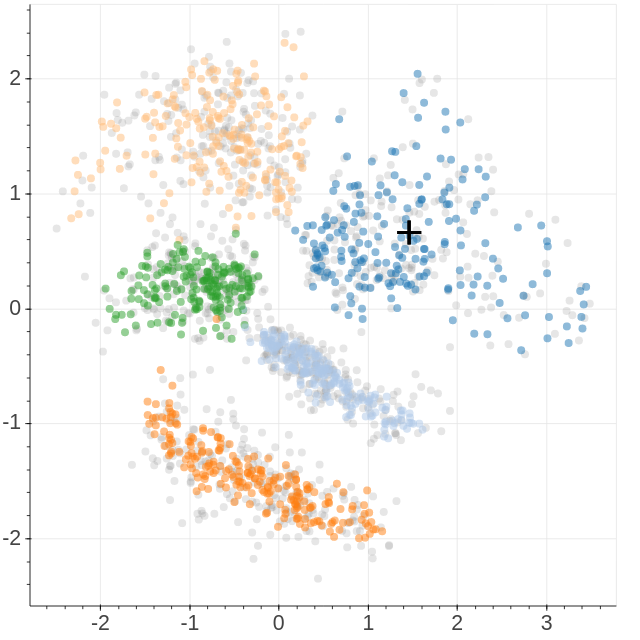
\includegraphics[height=4.5cm]{img/STEP1/ls3.png} \label{step1_3}}
    \subfigure{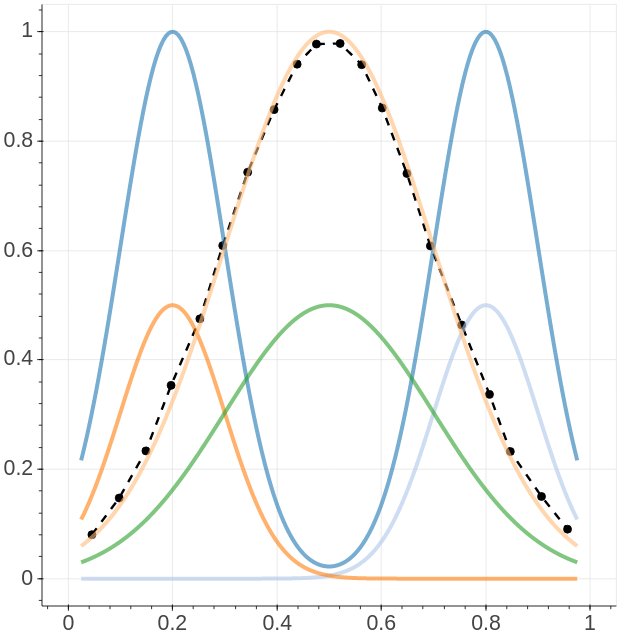
\includegraphics[height=4.5cm]{img/STEP1/gn1.png} \label{step1_4}}
    \subfigure{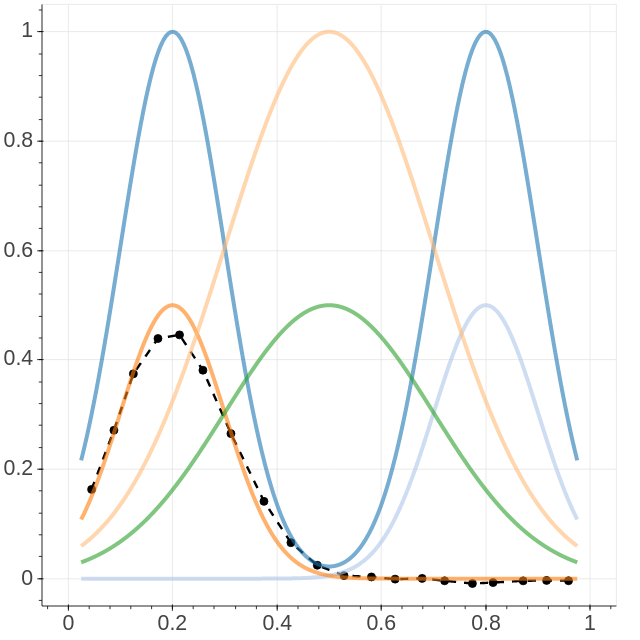
\includegraphics[height=4.5cm]{img/STEP1/gn2.png} \label{step1_5}}
    \subfigure{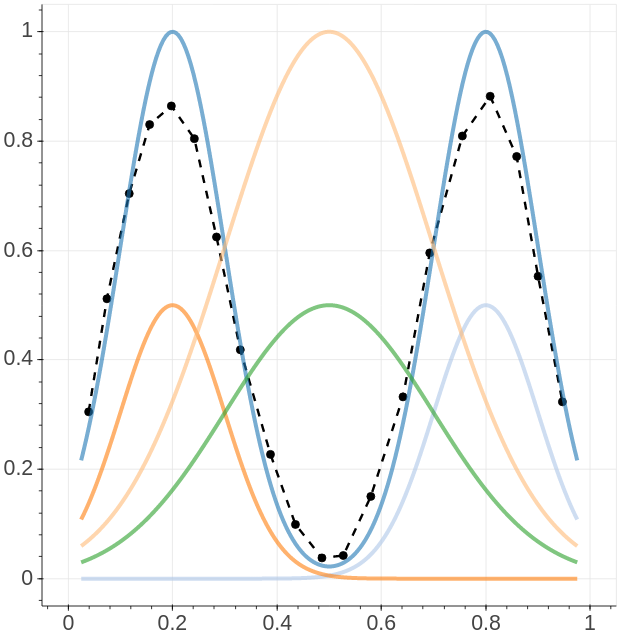
\includegraphics[height=4.5cm]{img/STEP1/gn3.png} \label{step1_6}}
    \caption{ STEP1 ls/gn }
    \label{fig:step_1}
\end{figure}


\section{Latent space regularization}

\section{Constraining regularizer with semi-supervised training}

% \chapter{Machine Learning and Latent Space Equilibrium}
% \section{Unsupervised learning: SVM and Autoencoders}
% \section{Variational autoencoders and ELBO minimization}
% \section{Latent space topology in a simulated world}
% \section{Latent space regularization}
% \section{Constraining regularizer with semi-supervised training}


\chapter{Embedded ML Infrastructure for Plasma Characterization}
\label{section:4_embedded_ML}

It has been shown in the introductory chapter the diversification of signals within their heterogeneous nature, however a particular discussion should be also addressed to the possible domain of the data itself beyond the particular origin.
In order to provide high quality descriptions of the plasma properties during a the pulse in a fusion experiment session a wide amount of sensors are usually required, both in time and in spatial domains.
Although it is not true that controllability (and observability) of the system strictly depends on that amount of inputs; the overall description of a complex system, indeed, is usually led by few driving signals~\cite{Liu2011}. 
This definition agrees with the intuitive notion of control that, for a properly structured system, the appropriate manipulation of a few state variables are a sufficient information to drive the whole behavior; like in the bike riding example where the actual only two control variable are the steering of the handlebar and the torque on the pedals. Even if the complete environment of all the variables that must be observed to provide a optimal control on the system states is rather complex, it can be shown that a properly configured latent variables can effectively generate a simpler embedded representation. This in turn leads to a simpler control model taking inputs from the latent states instead of directly depending on the whole detectors.

% CONTROL THEORY
According to the classical \textit{control theory} for dynamical systems, once the precise time derivative description is given in terms of that state space model, a system can be defined \textit{controllable} if there exist a particular set of inputs that are able to drive the state to any desired \textit{set point} within a finite time. 
If the classical discreet time \acl{LTI} state space model is considered in the form:
\begin{align}
    & \dot{\bm{x}} = A\bm{x} + B\bm{u} + \bm{w}\\
    & \bm{y} = C\bm{x} + D\bm{u} + \bm{v}
    \label{eq:ss_model}
\end{align}
% \begin{align}
%     & \bm{x}_t = A\bm{x}_{t-1} + B\bm{u}_t + \bm{w}_t\\
%     & \bm{y}_t = C\bm{x}_t + D\bm{u}_t + \bm{v}_t
%     \label{eq:ss_model}
% \end{align}

Time dependent state space models in \eqref{eq:ss_model}, also known \acl{DLM}, are a widely used approximation for analyzing time series. They provide a very flexible framework allowing concurrent smooth and steep changes that generally well fitting natural process time evolution.
A more rigorous formulation for \textit{controllability} is given in terms of the \textit{Kalman criterion}:
\begin{definition}{Kalman criterion}
The pair $(A,B)$ is \textit{controllable} if, given a duration $t>0$ and two arbitrary points $x_0, x_t \in \mathbb{R}^n$, there exists a piece wise continuous function $\tau \mapsto u(\tau)$ from $[0,t]$ to $\mathbb{R}^m$, such that the integral $x(\tau)$ generated from input $u$ with $x(0) = x_0$, satisfies $x(t)=x_t$.
\end{definition}
Where, as stated, the definition can be formulated in terms of the integral:
\begin{equation}
    e^{A t}x_0 + \int_0^t e^{A(t-\tau)}B u(\tau) d\tau = x_t
\end{equation}
where the only dependencies are on the state and input matrices $A$ and $B$.
Given the definition is well known that for such models the \textit{controllability} and the \textit{observability} depend on the \textit{Kalman condition}:
\begin{equation}
    \mathrm{rank}\,\mathscr{C} = \mathrm{rank}\left( B|AB|...|A^{n-1}B \right) = n
\end{equation}
% It can be shown that once a system is proved to be controllable can be transformed to a system in \textbf{canonical form} where all 

%% Structural Controllability
Recently, the study of the such complex networks with linear dynamics control has gained importance in both science and engineering. Between different aspects in which we can study the controllability we have the notion of structural controllability that has been proposed by Lin in~\cite{1100557} as a framework for studying the controllability properties of directed complex networks where
% LIN
%% RR
% To do this, the basic concept of a "cactus" and the related concept of a "precactus" are introduced. The main result of this paper states that the pair (A,b) is structurally controllable if an only if the graph of (A,b) is "spanned by a cactus." The result is also expressed in a more conventional way, in terms of some properties of the pair (A,b).

% \cite{zheng2017state}
State space models (SSMs), such as hidden Markov models (HMM) and linear dynamical systems
(LDS), have been the workhorse of sequence modeling in the past decades From a graphical model
perspective, efficient message passing algorithms (Stratonovich, 1960; Kalman, 1960) are available
in compact closed form thanks to their simple linear Markov structure. However, simplicity comes
at a cost: real world sequences can have long-range dependencies that cannot be captured by Markov
models; and the linearity of transition and emission restricts the flexibility of the model for complex
sequences.

As a first attempt the simple \textit{Elman} formulation for the recurrent topology will be applied, this with the aim at demonstrating the connection with linear dynamical systems, showing that such networks represent a superset.
With the \textit{Elman} forumlation a \acs{RNN} is control dynamical system that, in continuous time, can be described by a system of differential equations:
\begin{align}
    & \dot{\bm{x}} = \sigma_x \left( A\bm{x} + B\bm{u} \right) \\
    & \bm{y} = C\bm{x}
\end{align}
where for simplicity we omitted noise components for both the state and the output, and the direct input/output link.
% why



A popular alternative is the recurrent neural networks (RNN), for instance the Long Short-Term
Memory (LSTM) (Hochreiter  Schmidhuber, 1997) which has become a standard for sequence
modeling nowadays. Instead of associating the observations with stochastic latent variables, RNN
directly defines the distribution of each observation conditioned on the past, parameterized by a
neural network. The recurrent parameterization not only allows RNN to provide a rich function
class, but also permits scalable stochastic optimization such as the backpropagation through time
(BPTT) algorithm. However, flexibility does not come for free as well: due to the complex form of
the transition function, the hidden states of RNN are often hard to interpret. Moreover, it can require
large amount of parameters for seemingly simple sequence models (Zaheer et al., 2017).



\section{Easing the curse of dimensionality by disentangled factors}


\section{A new “smart” DAQ chain proposal}
% smart sensory
% feature extraction concept

In order to collect magnetic field measurements from EM probes, analog integration system~\cite{pomaro2005transducers} was implemented in RFX-mod, followed by two separate sets of ADC channels, one for precision off-line transient data and the other for real-time control. Re-implementing the same front-end for an increased number of channels is costly, requiring enhanced analog integration and duplication in ADC channels.  A more compact and cost effective solution is being investigated~\cite{gottardo18}, using a configurable FPGA to handle ADC conversion and providing a set of on-line functions directly performed at the FPGA logic level, including the numeric integration in real-time, recording at the same time the dB/dt signals deriving directly from EM coils needed to study the Magneto Hydro Dynamic (MHD) processes taking place into the plasma~\cite{zuin2009current}~\cite{innocente2014tearing}. The possibility of directly acquiring the time derivative of the electromagnetic fields, i.e. the direct signals from EM probes, was not present in the previous system, acquiring integrated signals in order to reduce the number of required ADC channels. This fact introduced a severe limitation in the derivative control required for MHD stabilization because of the bad quality of the computed time derivative.

The proposed approach will further reduce the number of ADC channels by merging high frequency transient recording in local memory (up to 1 MHz) and lower frequency streaming (up to 10 kHz) required for real-time plasma control and having a single ADC channel performing both. In RFX-mod a fixed subset of signals from EM probes was used for the active plasma control, requiring a new set of ADC converters in respect to the transient recorders used for data acquisition. In RFX-mod2 it will be possible to re-use any ADC channel from EM probes for real-time plasma control, being the actual number possibly limited by other factors not related to the ADC devices, such as network bandwidth or control computation load. 
%
The flexibility provided by a configurable on board FPGA allows also the inclusion of more sophisticated triggering mechanisms and a deeper integration with the timing systems. Examples of triggering mechanism are given by the acquisition of fast transients requiring high speed sampling only in a given, dynamic Region of Interest (ROI). This feature has been implemented in the first proof-of-concept device described in a later section. Deeper integration with the timing systems imply the ability of getting the clock and the trigger signals not only from digital inputs, but also from the specifically coded signal carrying both clock and trigger information (timing highway)\cite{dio4}. Such signals were used in the RFX-mod timing systems to distribute a synchronous clock and asynchronous triggers and a timing device was required for every ADC rack to extract the clock and the trigger signals. The timing device is no more required for a rack hosting the new ADC devices because the ADC devices can directly extract timing information from the timing highway.  
%
The adoption of a System on Chip (SoC) based technology exploiting both an ARM based processing unit and a FPGA logic provides the  flexibility of a configurable device for real-time operations and as well as the possibility of deploying software components directly on-board. The Red Pitaya board~\cite{redpitaya} is currently used for the development of the architecture. A different solution is however foreseen for the production system integrating an external ADC section with the Zynq-based SoC board. An ADC front end, already used in other applications of real-time plasma control~\cite{ATCA-MIMO-ISOL} was initially considered, but its noise characteristics, and in particular the noise dependency on frequency, proved to limit the quality of digital integration. For this reason, a different solution for the ADC stage is being considered.

The first implementation of the flexible ADC architecture has been carried out on a Red Pitaya board, using the in-board ADC channels. Even if not intended to represent the final application, development of FPGA logic on Red Pitaya offers the advantage of a ready-to-use ADC channel for development and first tests. Most of the firmware will be retained in the final implementation, using a different ADC front end. 
%
The time critical functions carried out by the FPGA in this context are:
\begin{itemize}
\item The management of a circular data buffer and the DMA transfer in RAM of pre and post trigger samples after the trigger has been received;
\item anti-aliasing filtering and subsequent sub-sampling of the samples to be streamed. The resulting samples are enqueued in a FIFO accessed by the processor;
\item digital integration for deriving magnetic field measurements from EM probe signals. Observe that in this case a single ADC stage will generate two ADC channels;
\item ROI detection in case ADC triggers are derived from the signal itself (e.g. over a given signal level threshold);
\item Clock and trigger extraction in case a highway signal is provided by the timing system, encoding both clock an triggers.
\end{itemize}
%
The less critical functions that will be carried out by the processor unit are:
\begin{itemize}
\item The management of the configuration setting, received via TCP/IP or HTTP. The processor validates the configuration and write the appreciate registers in the FPGA;
\item off-line data readout of acquired samples in transient recording and communication via TCP/IP with the central data acquisition system;
\item network data streaming of sub-sampled data read from the FIFO and sent in UDP packets to the active plasma control system. 
\end{itemize}
%
In addition to pre-configured blocks from the XILINX toolbox for data buffering, DMA engine, I/O FIFO and registers, three blocks implemented in VHDL carry out the underlying logic. The first block provides the management of clock and triggers that may be either directly derived from digital inputs or rebuild by properly decoding the timing highway input signal. The second block provides programmable input signal elaboration such as low pass filtering for subsampling and integration. The third block will handle the triggering logic and the circular buffer holding pre and post trigger samples. In particular, the trigger may be derived from external signals (via the first block) or derived from the input signal (e.g. when the input level is greater than a given threshold).    

Communication of subsamples streamed data for real-time plasma control is achieved using the XILINX AXI Stream FIFO. The Xilinx AXI Stream FIFO is a Xilinx free software IP that implement a read/write FIFO queue with a well defined communication protocol. A proper connected IRQ line is used to trigger events to the processing unit together with the related set of status and enable registers. In this way data samples are readily available to the linux processor and will be sent using low latency UDP communication to computing nodes carrying out distributed for real-time plasma control. Communication of the data acquired at high speed in the ROI is carried out by a DMA engine, using circular DMA buffers in order to minimize the number of data copies. In this case data will be sent to the central Data Acquisition system via TCP/IP as soon as a ROI has been acquired. Fig. 1 shows the main blocks of the ADC device: the external ADC circuitry, communicating with the FPGA via a serial LVDS link; the FPGA logic, communicating with the processor via registers, FIFO and DMA; the processor components, in kernel and user space. 
~
~
\begin{figure}[ht]
\centering
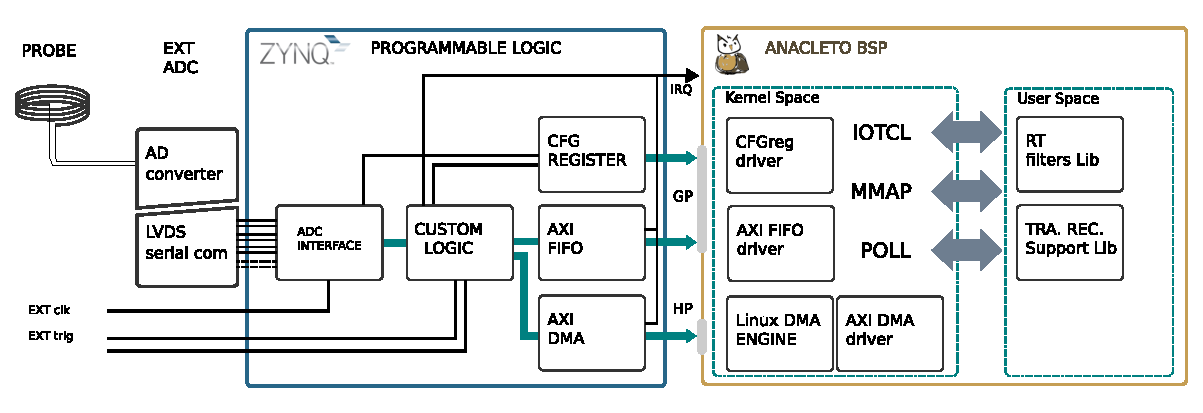
\includegraphics[width=0.9\textwidth]{img/4_EmbeddedML/schema_logico.pdf}
\caption{Logic design of the flexible ADC structure.}
\label{fig:logic}
\end{figure}









\section{Quantized neural networks for embedded implementation}

In numerical computation we refer to the \textit{quantization} as the process of constraining the number of bit that reproduce a numerical value. In effect any digital number is already intrinsically quantized, in the sense that its representation is defined on a limited discreet domain. Nevertheless, even if the number of bits that are used to represent a digital quantity is finite, and so is the possible set of values that it can assume, the actual position of those values in the target domain is not strictly fixed. This means that we can decide where to place any of possible available reproduction number to fit the desired manifold.
If the function that maps the digital representation with a numerical entity is linear the numerical format can be described by only two parameters: the \textbf{range}, which refers to the range of all possible numbers that can be represented, and the \textbf{precision} that tells how many values can be represented within the dynamic range, which in turn determines the resolution (the distance in the target domain between two adjacent numbers).

In the context of deep learning, and in information theory in general, the predominant numerical format used for both training and final deployment is the floating point, either in 32-bits or 64-bits versions. For a \acs{MLP}, for example, floating point operations involves the linear combination of weights and biases with input features for each layer, and the non-linear activation function. The formulation of floating point numerical format is a very clever solution that adapt the range to the represented number.

Floating-point can be thought in concept similar to the scientific notation. Their numbers consist of a signed set of digits of a fixed length in a given base (the radix), this is referred as the \textit{significand}; where its length determines the precision to which numbers can be represented. The radix point position is assumed always to be within the significand, while a signed integer exponent modifies the magnitude of the number.
To finally derive the actual value of the floating-point number the significand is multiplied by the base and raised to the power of the exponent; this is shifting the radix point from its implied position by a number of places equal to the value of the exponent to the right if the exponent is positive or to the left if the exponent is negative.
%
Symbolically, this represented value can be derived as:
\begin{equation*}
    \frac{s}{b^{p-1}} \times b^e
\end{equation*}
where $s$ is the significand, $p$ is the precision (the number of digits in the significand), $b$ is the base, and $e$ is the exponent.
The flexibility introduced by floating point dynamic range is that the numbers that can be represented are not uniformly spaced; the difference between two consecutive representable numbers grows with the chosen scale.

However given this dynamic mapping of the scale the floating point may require a slight amount of computational resources.
When a processing unit is executing an algorithm where a floating-point operation is not directly supported by the hardware, the CPU tries to use a series of simpler floating-point operations, either by basic internal routines or by means of specific libraries. In systems without any floating-point hardware, the CPU emulates it using a series of simpler fixed-point arithmetic operations that run on the integer arithmetic logic unit.
Moreover, being the target a possible FPGA implementation, the full IEEE 754 floating point shown to use a lot of hardware resources in terms of LUTs counts. 

The desire for reduced bandwidth and compute requirements of deep learning models has driven research into using lower-precision numerical formats. It has been largely proved that both linear combination and non linear activation can be effectively represented using a fixed point math, in particular 8-bit integers (INT8) have been successfully applied without incurring in significant loss of accuracy. 
But, not enough, the use of even lower bit-widths, such as 4/2/1-bits, is an active field of research that has also shown great results.


% \chapter{Embedded ML Infrastructure for Plasma Characterization}
% \section{A new “smart” DAQ chain proposal for features extraction ( lavoro con Marco Gottardo )}
% \section{Easing the curse of dimensionality by means of latent space compression}
% \section{Quantized neural networks for embedded implementation and the Xilinx FINN package}

\chapter{Mildstone implementation details}
\section{Anacleto - Mildstone component for embedded FPGA development}
\section{Kinds of communication channel}
\section{Tensorflow with external proxy}
\section{Mim - Mildstone approach for interface modelling}

% \chapter{Mildstone implementation details}
% \section{Anacleto - Mildstone component for embedded FPGA development}
% \section{Kinds of communication channel}
% \section{Tensorflow with external proxy}
% \section{Mim - Mildstone approach for interface modelling}

\chapter{RFX-Hunch: a closed example based on electron temperature}
\label{section:RFXhunch}

\section{What involved ( basing on “SCHEMA” )} % SHAx
%% FD-NT-27
\section{Passing from simulated data to actual data  “missing points”  }


\section{( show using of dropout, rebalancing and beta )}


\section{Adding information through models ( Zanca-Terranova )}


\section{parameters to SXR mapping}

\subsection{STEP 12.7}

\begin{figure}
    \centering
    \subfigure{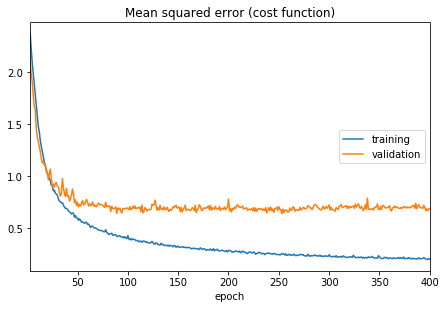
\includegraphics[height=3.3cm]{img/STEP12_7/STEP12_7_pBr2SXR_rm-rs_absarg_training_mse.png} \label{step_12_7_training}}
    \subfigure{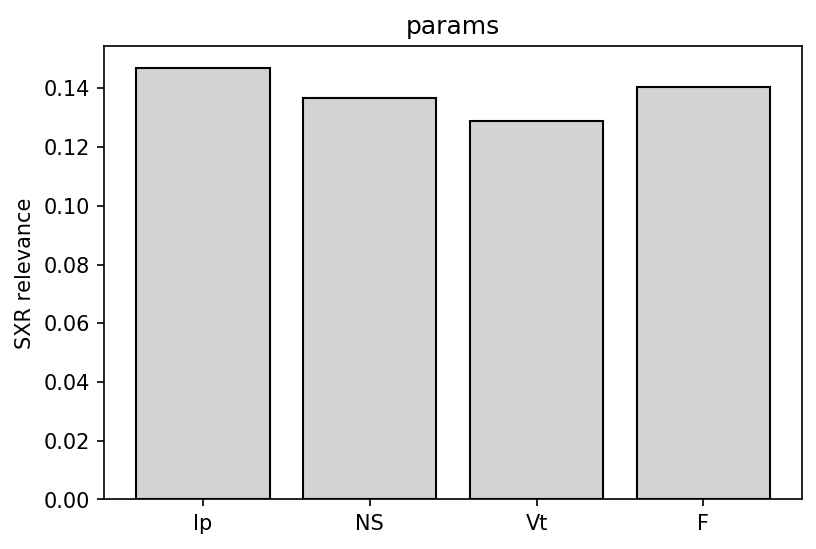
\includegraphics[height=3.3cm]{img/STEP12_7/STEP12_7_params.png} \label{step_12_7_p}}
    \subfigure{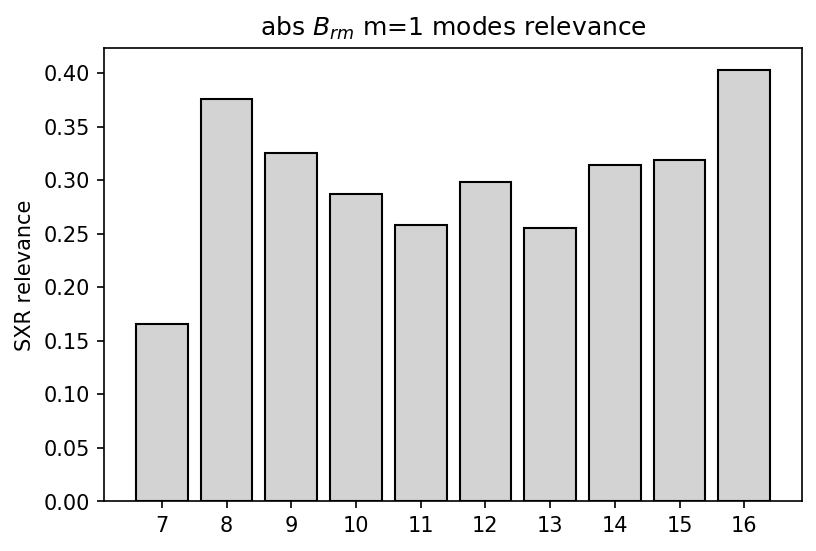
\includegraphics[height=3.3cm]{img/STEP12_7/STEP12_7_abs_Br_rm.png} \label{step_12_7_abs_Brm}}
    \subfigure{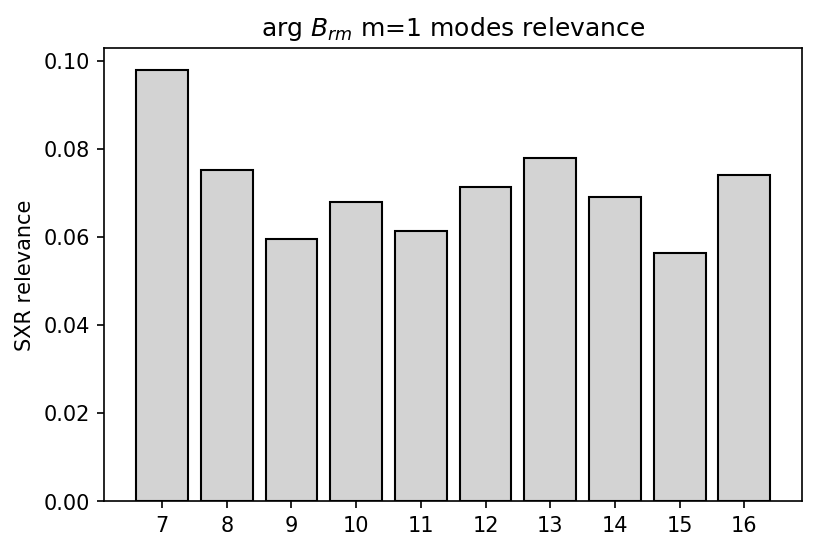
\includegraphics[height=3.3cm]{img/STEP12_7/STEP12_7_arg_Br_rm.png} \label{step_12_7_arg_Brm}}
    \subfigure{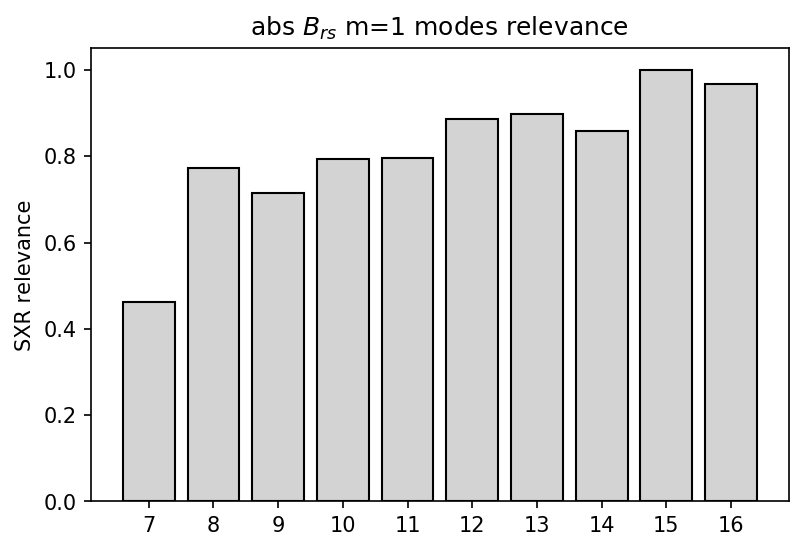
\includegraphics[height=3.3cm]{img/STEP12_7/STEP12_7_abs_Br_rs.png} \label{step_12_7_abs_Brs}}
    \subfigure{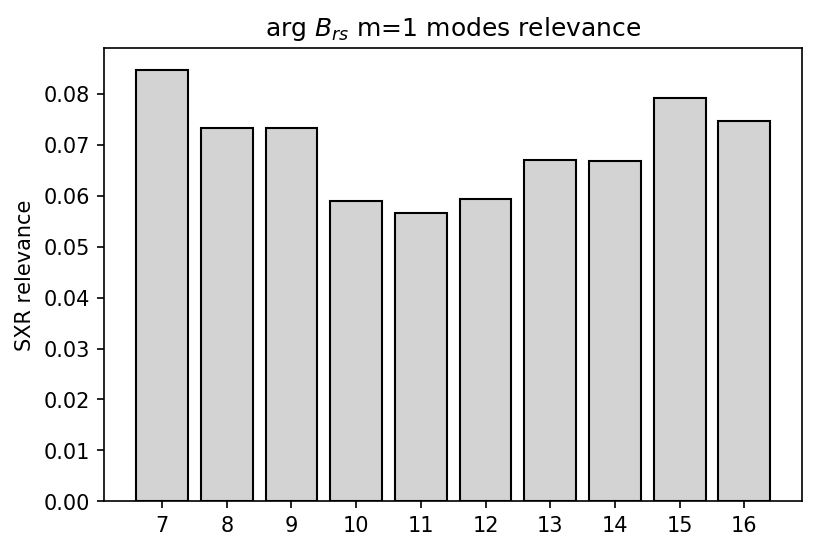
\includegraphics[height=3.3cm]{img/STEP12_7/STEP12_7_arg_Br_rs.png} \label{step_12_7_arg_Brs}}
    \caption{ Training 500 epochs - STEP 12.7 mse, slightly overfitted but validation not diverging }
    \label{fig:step_12_7}
\end{figure}

\begin{figure}
    \centering
    \subfigure{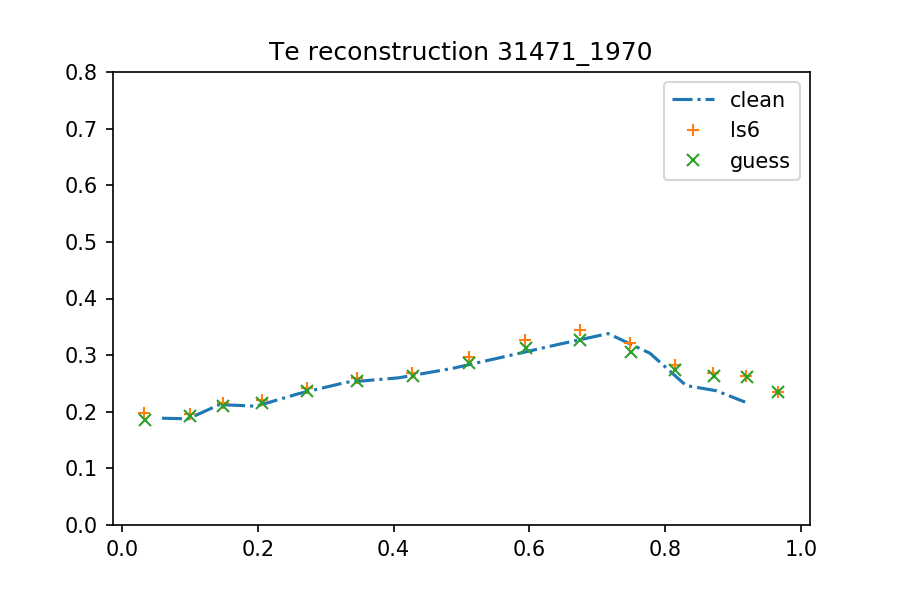
\includegraphics[height=4.8cm]{img/STEP12_7/Te_rec_215.png} }
%   \subfigure{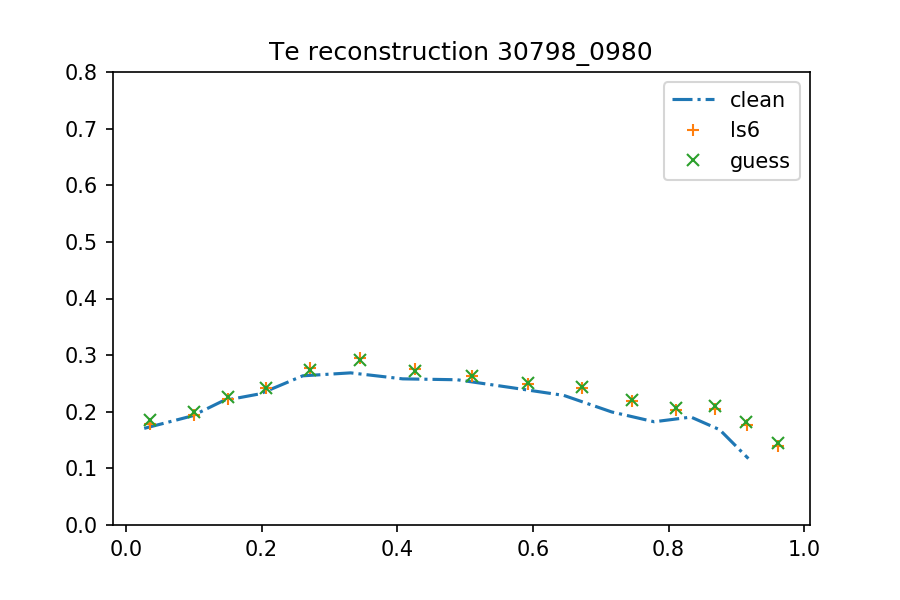
\includegraphics[height=4.8cm]{img/STEP12_7/Te_rec_219.png} }
    \subfigure{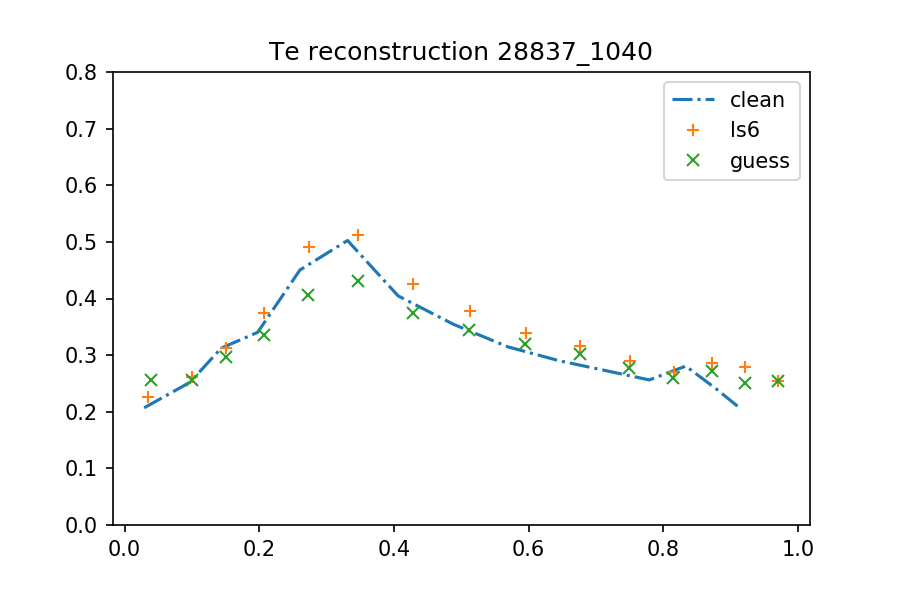
\includegraphics[height=4.8cm]{img/STEP12_7/Te_rec_229.png} }
    \subfigure{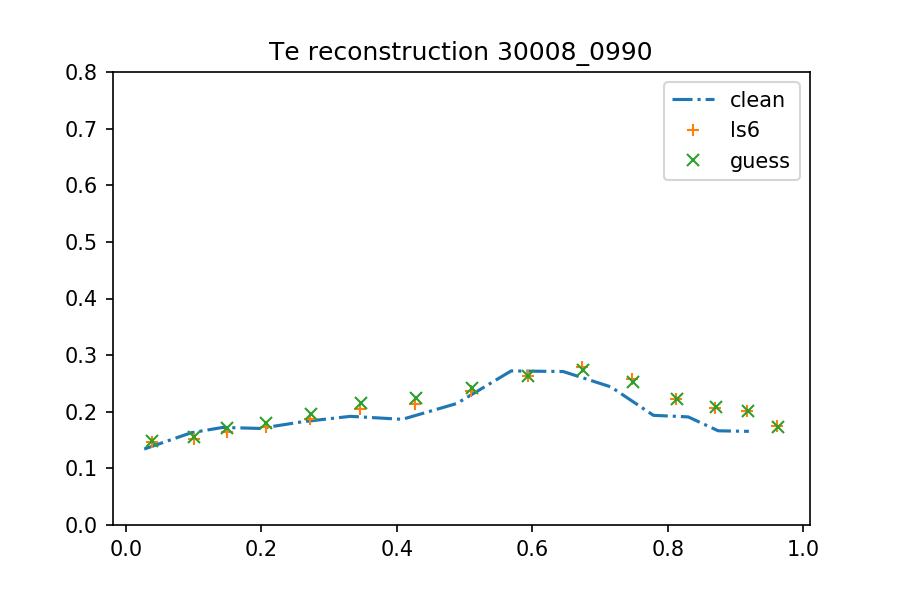
\includegraphics[height=4.8cm]{img/STEP12_7/Te_rec_232.png} }
%   \subfigure{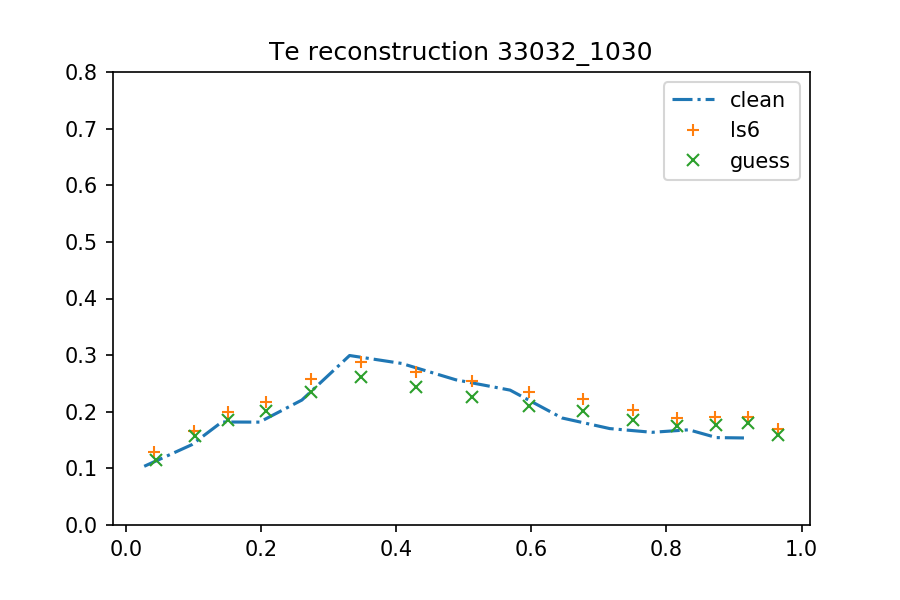
\includegraphics[height=4.8cm]{img/STEP12_7/Te_rec_243.png} }
    \subfigure{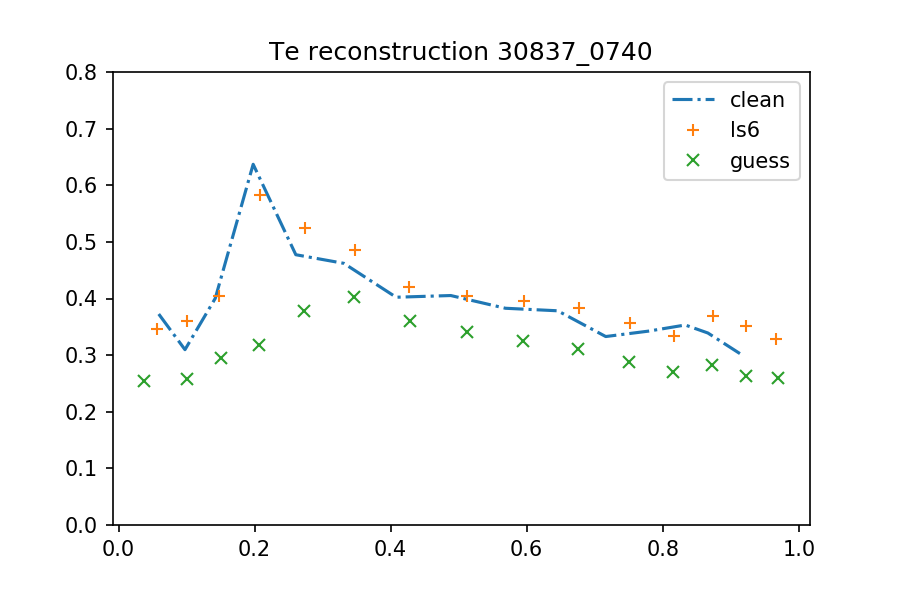
\includegraphics[height=4.8cm]{img/STEP12_7/Te_rec_213.png} }
    \caption{ Training 500 epochs - STEP 12.7 mse, slightly overfitted but validation not diverging }
    \label{fig:step_12_7_rec}
\end{figure}


% \chapter{T-Hunch: a closed example based on electron temperature}
% \section{What involved ( basing on “SCHEMA” )}
% \section{Passing from simulated data to actual data  “missing points”  }
% \section{( show using of dropout, rebalancing and beta )}
% \section{Adding information through models ( Zanca-Terranova )}

\chapter{Results}
\section{If any}

\chapter{Conclusions}

\chapter{Appendix}
\section{Projects that are already there built upon Anacleto:}
\subsection{W7X - trigger }
\subsection{NIO fast daq}
\subsection{Spider Redpitaya}
\section{Projects that are already there built upon Tensorflow:}
\subsection{Jasper and Horace }

\printindex

%% ACRONYMS %%
\newpage
\chapter*{List of acronyms}
\begin{acronym}

%% MACHINE LEARNING %%
\acro{AI}{\emph{Artificial Intelligence}}
\acro{ML}{\emph{Machine Learning}}
\acro{ANN}{\emph{Artificial Neural Networks}}
\acro{DNN}{\emph{Deep Neural Networks}}
\acro{CNN}{\emph{Convolutional Neural Networks}}
\acro{ELBO}{}
\acro{GLM}{Generalized Linear Model}
\acro{MLP}{Multi-Layer Perceptron}
\acro{HMM}{Hidden Markov Model}
\acro{ABM}{Adaptive Basis Function Model}

%% PLASMA
\acro{RFP}{Reverse Field Pinch}
\acro{MHD}{Magneto-hydro dynamics}
% \acro{CNR}{Consiglio Nazionale delle Ricerche}
% \acro{INFN}{Istituto Nazionele di Fisica Nucleare}
% \acro{ENEA}{Italian National Agency for New Technologies, Energy and Sustainable Economic Development}

%% HARDWARE
\acro{FPGA}{field-programmable gate array}
\acro{CPU}{Central Processing Unit}
\acro{GPU}{Graphic Processing Unit}
\acro{TPU}{Tensor Processing Unit}
\acro{RTL}{Register Transfer Level}
\acro{HDL}{Hardware description Language}

\acro{ADC}{Analog to Digital Converter}
\acro{DAQ}{Data Aquisition system}


\end{acronym}


%% BIBLIOGRAPHY %%
\newpage
\bibliographystyle{unsrt}
\bibliography{bib/ML,bib/plasma,bib/rfx,bib/spider}
\end{document}
